%!TEX root = ../larxxia.tex


\section{Factorise to the singular value decomposition}
\label{sec:fisvd}
\secttoc

\begin{comment}
\pooliv{\S7.4} \holti{\S8.4} \cite[\S06]{Davis99a} \cite[\S8.7]{Nakos1998}
In a sense, the \svd\ replaces the \(\tr PLU\) factorisation of classic linear algebra, e.g.\ \pooliv{\S3.4}.
The computation of an \svd\ is well conditioned, unlike \textsc{lu} decomposition and eigenvalue calculations which are commonly poorly conditioned.
\end{comment}


The singular value decomposition (\svd) is sometimes called the \idx{jewel in the crown} of  linear algebra.
%It is a vital part of the toolkit needed by many scientists, engineers, statisticians and mathematicians.
\begin{aside}
Beltrami first derived the \svd\ in 1873.  
The first reliable method for computing an \svd\ was developed by Golub and Kahan in 1965, and only thereafter did applications proliferate.
\end{aside}
Its importance is certified by the many names by which it is invoked in scientific and engineering applications: principal component analysis, singular spectrum analysis, principal orthogonal decomposition, latent semantic indexing, Schmidt decomposition, correspondence analysis, Lanczos methods, dimension reduction, and so on.
Let's start seeing what it can do for us.




\subsection{Introductory examples}
\label{sec:svdeg}

You are a contestant in a quiz show.
The final million dollar question is: 
\begin{aside}
Introduce an analogous problem so the \svd\ procedure follows more easily.
\end{aside}
\begin{quote}
in your head, without a calculator, solve \(42\,x=1554\) within twenty seconds,
\end{quote} 
your time starts now\dotfill
\begin{solution} 
Long division is hopeless in the time available.  
However, recognise \(42=2\cdot3\cdot7\) and so divide 1554 by~2 to get~777, divide 777 by~3 to get~259, and divide 259 by~7 to get~37, and win the prize.
\end{solution}

\begin{activity} \label{eg:}
Given \(154=2\cdot7\cdot11\)\,, solve in your head \(154x=8008\) or~\(9856\) or~\(12628\) or~\(13090\) or~\(14322\) (teacher to choose): first to answer wins.
\end{activity}

Such examples show \idx{factorisation} can turn a hard problem into a sequence of easy problems.  
We adopt an analogous matrix factorisation to solve and understand general linear equations.  

To illustrate the procedure to come, let's write the above solution steps in detail: we solve \(42x=1554\)\,.
\begin{enumerate}
\item Factorise the coefficient \(42=2\cdot3\cdot7\) so the equation becomes  
\begin{equation*}
2\cdot\underbrace{3\cdot\overbrace{7x}^{=y}}_{=z}=1554\,,
\end{equation*}
and introduce two intermediate unknowns \(y\) and~\(z\) as shown above.
\item Solve \(2z=1554\) to get \(z=777\)\,.
\item Solve \(3y=z=777\) to get \(y=259\)\,.
\item Solve \(7x=y=259\) to get \(x=37\)\,---the answer.
\end{enumerate}

Now let's proceed to small matrix examples to introduce the general matrix procedure empowered by the factorisation of a singular value decomposition (\svd).
%\begin{comment}
%Other possible similar matrices are (transposes)
%[5,5;1,7]
%[7,4;1,8]
%[7,6;2,9]
%[8,1;4,7]
%[9,7;3,11]
%[9,8;1,12]
%\end{comment}
\begin{example} \label{eg:2by2svd}
Solve the \(2\times2\) system
\begin{equation*}
\begin{bmatrix} 10&2\\5&11 \end{bmatrix}\xv
=\begin{bmatrix} 18\\-1 \end{bmatrix}
\end{equation*}
given the matrix factorisation
\begin{equation*}
\begin{bmatrix} 10&2\\5&11 \end{bmatrix}=
\begin{bmatrix} \frac35&-\frac45\\\frac45&\frac35 \end{bmatrix}
\begin{bmatrix} 10\sqrt2&0\\0&5\sqrt2 \end{bmatrix}
\tr{\begin{bmatrix} \frac1{\sqrt2}&-\frac1{\sqrt2}\\ \frac1{\sqrt2}&\frac1{\sqrt2} \end{bmatrix}}
\end{equation*}
(note the transpose on the last matrix).
\begin{solution} 
Optionally check the factorisation if you like:
\begin{eqnarray*}&&
\begin{bmatrix} \frac35&-\frac45\\\frac45&\frac35 \end{bmatrix}
\begin{bmatrix} 10\sqrt2&0\\0&5\sqrt2 \end{bmatrix}
=\begin{bmatrix} 6{\sqrt2}& -4{\sqrt2}
\\ 8{\sqrt2}&3{\sqrt2} \end{bmatrix};
\\\text{then}&&
\begin{bmatrix} 6{\sqrt2}& -4{\sqrt2}
\\ 8{\sqrt2}&3{\sqrt2} \end{bmatrix}
\begin{bmatrix} \frac1{\sqrt2}&\frac1{\sqrt2}\\ -\frac1{\sqrt2}&\frac1{\sqrt2} \end{bmatrix}
=\begin{bmatrix} 10&2\\5&11 \end{bmatrix}.
\end{eqnarray*}
Given the factorisation, the following four steps forms the general procedure. 
\begin{enumerate}
\item Write the system using the factorisation, and with two intermediate unknowns~\yv\ and~\zv:
\begin{equation*}
\begin{bmatrix} \frac35&-\frac45\\\frac45&\frac35 \end{bmatrix}
\underbrace{\begin{bmatrix} 10\sqrt2&0\\0&5\sqrt2 \end{bmatrix}
\overbrace{\tr{\begin{bmatrix} \frac1{\sqrt2}&-\frac1{\sqrt2}\\ \frac1{\sqrt2}&\frac1{\sqrt2} \end{bmatrix}}\xv}^{=\yv}}_{=\zv}=\begin{bmatrix} 18\\-1 \end{bmatrix}.
\end{equation*}

\item Solve \(\begin{bmatrix} \frac35&-\frac45\\\frac45&\frac35 \end{bmatrix}\zv=\begin{bmatrix} 18\\-1 \end{bmatrix}\)\,: recall that the matrix appearing here is orthogonal (and this orthogonality is no accident), so multiplying by the transpose gives the intermediary
\begin{equation*}
\zv=\begin{bmatrix} \frac35&\frac45\\-\frac45&\frac35 \end{bmatrix}
\begin{bmatrix} 18\\-1 \end{bmatrix}
=\begin{bmatrix} 10\\-15 \end{bmatrix}.
\end{equation*}

\item Now solve \(\begin{bmatrix} 10\sqrt2&0\\0&5\sqrt2 \end{bmatrix}\yv=\zv=\begin{bmatrix} 10\\-15 \end{bmatrix}\)\,:  the matrix appearing here is diagonal (and this is no accident), so dividing by the respective diagonal elements gives the intermediary
\begin{equation*}
\yv=\begin{bmatrix} 10\sqrt2&0\\0&5\sqrt2 \end{bmatrix}^{-1}
\begin{bmatrix} 10\\-15 \end{bmatrix}
=\begin{bmatrix} 1/\sqrt2\\-3/\sqrt2 \end{bmatrix}.
\end{equation*}

\item Finally solve \(\tr{\begin{bmatrix} \frac1{\sqrt2}&-\frac1{\sqrt2}\\ \frac1{\sqrt2}&\frac1{\sqrt2} \end{bmatrix}}\xv=\yv=\begin{bmatrix} 1/\sqrt2\\-3/\sqrt2 \end{bmatrix}\)\,: now the matrix appearing here is also orthogonal (this orthogonality is also no accident), so multiplying by itself (the transpose of the transpose) gives the solution
\begin{equation*}
\xv=\begin{bmatrix} \frac1{\sqrt2}&-\frac1{\sqrt2}\\ \frac1{\sqrt2}&\frac1{\sqrt2} \end{bmatrix}
\begin{bmatrix} 1/\sqrt2\\-3/\sqrt2 \end{bmatrix}
=\begin{bmatrix} \frac12+\frac32\\\frac12-\frac32 \end{bmatrix}
=\begin{bmatrix} 2\\-1 \end{bmatrix}.
\end{equation*}

\end{enumerate}
\end{solution}
\end{example}





\begin{activity}
Let's solve the system \(\begin{bmatrix} 12&-41\\34&-12 \end{bmatrix}\xv=\begin{bmatrix} 94\\58 \end{bmatrix}\) using the factorisation
\begin{equation*}
\begin{bmatrix} 12&-41\\34&-12 \end{bmatrix}
=\begin{bmatrix} \frac45&-\frac35\\\frac35&\frac45 \end{bmatrix}
\begin{bmatrix} 50&0\\0&25 \end{bmatrix}
\tr{\begin{bmatrix} \frac35&\frac45\\-\frac45&\frac35 \end{bmatrix}}
\end{equation*}
in which the first and third matrices on the right-hand side are orthogonal. 
After solving \(\begin{bmatrix} \frac45&-\frac35\\\frac35&\frac45 \end{bmatrix}\zv=\begin{bmatrix} 94\\58 \end{bmatrix}\), the next step is to solve which of the following?
\begin{parts}
\item \(\begin{bmatrix} 50&0\\0&25 \end{bmatrix}\yv=\begin{bmatrix} 110\\-10 \end{bmatrix}\)
\item \(\begin{bmatrix} 50&0\\0&25 \end{bmatrix}\yv=\begin{bmatrix} \frac{202}5\\\frac{514}5 \end{bmatrix}\)
\item \(\begin{bmatrix} 50&0\\0&25 \end{bmatrix}\yv=\begin{bmatrix}  \frac{514}5\\-\frac{202}5 \end{bmatrix}\)
\item \(\begin{bmatrix} 50&0\\0&25 \end{bmatrix}\yv=\begin{bmatrix} 10\\110 \end{bmatrix}\)
\end{parts}
\end{activity}






\begin{example} \label{eg:3by3svd}
Solve the \(3\times3\) system
\begin{equation*}
A\xv=\begin{bmatrix} 10\\2\\-2 \end{bmatrix}
\quad\text{for matrix }A=\begin{bmatrix}-4&-2&4
\\-8&-1&-4
\\6&6&0\end{bmatrix}
\end{equation*}
using the following given matrix factorisation (note the last is transposed)
\begin{equation*}
A=\begin{bmatrix} \frac13&-\frac23&\frac23
\\\frac23&\frac23&\frac13
\\-\frac23&\frac13&\frac23 \end{bmatrix}
\begin{bmatrix} 12&0&0\\0&6&0\\0&0&3 \end{bmatrix}
\tr{\begin{bmatrix} -\frac89&-\frac19&-\frac49
\\-\frac49&\frac49&\frac79
\\-\frac19&-\frac89&\frac49 \end{bmatrix}}.
\end{equation*}

\begin{solution} 
Use \script.
Enter the matrices and the right-hand side, and check the factorisation (and the typing):
\setbox\ajrqrbox\hbox{\qrcode{% check SVD
U=[1,-2,2;2,2,1;-2,1,2]/3
S=[12,0,0;0,6,0;0,0,3]
V=[-8,-1,-4;-4,4,7;-1,-8,4]/9
b=[10;2;-2]
A=U*S*V'
}}%
\marginpar{\usebox{\ajrqrbox\\[2ex]}}%
\begin{verbatim}
U=[1,-2,2;2,2,1;-2,1,2]/3
S=[12,0,0;0,6,0;0,0,3]
V=[-8,-1,-4;-4,4,7;-1,-8,4]/9
b=[10;2;-2]
A=U*S*V'
\end{verbatim}
\begin{enumerate}
\item  Write the system \(A\xv=\bv\) using the factorisation, and with two intermediate unknowns~\yv\ and~\zv:
\begin{equation*}
\begin{bmatrix} \frac13&-\frac23&\frac23
\\\frac23&\frac23&\frac13
\\-\frac23&\frac13&\frac23 \end{bmatrix}
\underbrace{\begin{bmatrix} 12&0&0\\0&6&0\\0&0&3 \end{bmatrix}
\overbrace{\tr{\begin{bmatrix} -\frac89&-\frac19&-\frac49
\\-\frac49&\frac49&\frac79
\\-\frac19&-\frac89&\frac49 \end{bmatrix}}\xv}^{=\yv}}_{=\zv}=\begin{bmatrix} 10\\2\\-2 \end{bmatrix}.
\end{equation*}

\item Solve \(\begin{bmatrix} \frac13&-\frac23&\frac23
\\\frac23&\frac23&\frac13
\\-\frac23&\frac13&\frac23 \end{bmatrix}\zv=\begin{bmatrix} 10\\2\\-2 \end{bmatrix}\)\,. 
Now this matrix, called~\verb|U|, is orthogonal---check by computing~\verb|U'*U|---so multiplying by the transpose gives the intermediary: \(\verb|z=U'*b|=(6,-6,6)\).

\item Then solve \(\begin{bmatrix} 12&0&0\\0&6&0\\0&0&3 \end{bmatrix}\yv=\zv=\begin{bmatrix} 6\\-6\\6 \end{bmatrix}\)\,:  this matrix, called~\verb|S|, is diagonal, so dividing by the respective diagonal elements gives the intermediary \(\verb|y=z./diag(S)|=(\frac12,-1,2)\).

\item Finally solve \(\tr{\begin{bmatrix} -\frac89&-\frac19&-\frac49
\\-\frac49&\frac49&\frac79
\\-\frac19&-\frac89&\frac49 \end{bmatrix}}\xv=\yv=\begin{bmatrix} \frac12\\-1\\2 \end{bmatrix}\)\,. 
This matrix, called~\verb|V|, is also orthogonal---check by computing~\verb|V'*V|---so multiplying by itself (the transpose of the transpose) gives the final solution
\(\verb|x=V*y|=(-\frac{11}9,\frac89,\frac{31}{18})\).

\end{enumerate}
\end{solution}
\end{example}




\paragraph{Warning: do \emph{not} solve in reverse order} \ 
\begin{example} \label{eg:}
Reconsider Example~\ref{eg:2by2svd} wrongly.
\begin{enumerate}
\item 
After writing the system using the \svd\ as
\begin{equation*}
\begin{bmatrix} \frac35&-\frac45\\\frac45&\frac35 \end{bmatrix}
\underbrace{\begin{bmatrix} 10\sqrt2&0\\0&5\sqrt2 \end{bmatrix}
\overbrace{\tr{\begin{bmatrix} \frac1{\sqrt2}&-\frac1{\sqrt2}\\ \frac1{\sqrt2}&\frac1{\sqrt2} \end{bmatrix}}\xv}^{=\yv}}_{=\zv}=\begin{bmatrix} 18\\-1 \end{bmatrix},
\end{equation*}
one might be inadvertently tempted to `solve' the system by using the matrices in reverse order as in the following: \emph{do not do this}.

\item First solve \(\tr{\begin{bmatrix} \frac1{\sqrt2}&-\frac1{\sqrt2}\\ \frac1{\sqrt2}&\frac1{\sqrt2} \end{bmatrix}}\xv=\begin{bmatrix} 18\\-1 \end{bmatrix}\)\,:  this matrix is orthogonal, so multiplying by itself (the transpose of the transpose) gives 
\begin{equation*}
\xv=\begin{bmatrix} \frac1{\sqrt2}&-\frac1{\sqrt2}\\ \frac1{\sqrt2}&\frac1{\sqrt2} \end{bmatrix}
\begin{bmatrix} 18\\-1 \end{bmatrix}
=\begin{bmatrix} 19/\sqrt2\\17/\sqrt2 \end{bmatrix}.
\end{equation*}

\item Inappropriately `solve' \(\begin{bmatrix} 10\sqrt2&0\\0&5\sqrt2 \end{bmatrix}\yv=\begin{bmatrix} 19/\sqrt2\\17/\sqrt2 \end{bmatrix}\)\,:  this matrix is diagonal, so dividing by the diagonal elements gives 
\begin{equation*}
\yv=\begin{bmatrix} 10\sqrt2&0\\0&5\sqrt2 \end{bmatrix}^{-1}
\begin{bmatrix} 19/\sqrt2\\17/\sqrt2 \end{bmatrix}
=\begin{bmatrix} \frac{19}{20}\\\frac{17}{10} \end{bmatrix}.
\end{equation*}

\item Inappropriately `solve' \(\begin{bmatrix} \frac35&-\frac45\\\frac45&\frac35 \end{bmatrix}\zv=\begin{bmatrix} \frac{19}{20}\\\frac{17}{10} \end{bmatrix}\)\,: this matrix is orthogonal, so multiplying by the transpose gives 
\begin{equation*}
\zv=\begin{bmatrix} \frac35&\frac45\\-\frac45&\frac35 \end{bmatrix}
\begin{bmatrix} \frac{19}{20}\\\frac{17}{10} \end{bmatrix}
=\begin{bmatrix} 1.93\\0.26 \end{bmatrix}.
\end{equation*}
And then, since the solution is to be called~\xv, we might inappropriately call what we just calculated as the solution \(\xv=(1.93,0.26)\).
\end{enumerate}
\end{example}
Avoid this reverse process as it is wrong.
Matrix multiplicative is \emph{not} commutative (section~\ref{sec:fapmo}).  
We must use an \svd\ factorisation in the correct order: to solve linear equations use the matrices in an \svd\ from left to right.





\subsection{The SVD solves general systems}
\label{sec:svdsgs}

The previous examples depended upon a matrix being factored into a product of three matrices: two orthogonal and one diagonal.
\begin{aside}\url{http://www.youtube.com/watch?v=JEYLfIVvR9I} is an entertaining prelude.\end{aside}%
Amazingly, such factorisation is always possible.

\begin{theorem}[\svd\ factorisation] \label{thm:svd} 
    Every $m\times n$ real matrix~$A$ can be factored into a product of three matrices
    \begin{equation}
        A=\usv\,,
    \end{equation}
    called a \bfidx{singular value decomposition} (\svd), where
    \begin{itemize}
		\item $m\times m$ matrix~$U=\begin{bmatrix} \uv _1 &\uv_2&\cdots&\uv _m \end{bmatrix}$ is orthogonal\index{orthogonal matrix}, 
		\item $n\times n$ matrix~$V=\begin{bmatrix} \vv_1 &\vv_2&\cdots&\vv_n \end{bmatrix}$ is orthogonal\index{orthogonal matrix}, and      
        \item  $m\times n$ diagonal matrix~$S$ is zero except for non-negative diagonal elements called \bfidx{singular value}s
\begin{aside}
The greek letter~\(\sigma\) (sigma) denotes the singular values.
\end{aside}%
\hlist\sigma\mn, which are unique when ordered from largest to smallest so that $\sigma_1\geq \sigma_2 \geq \cdots \geq \sigma_{\mn}\geq 0$\,.
    \end{itemize}
    The \idx{orthonormal} vectors \(\uv_j\) and~\(\vv_j\) are called \bfidx{singular vector}s.
    \footnote{This enormously useful theorem also generalises from \(m\times n\) matrices to analogues in `infinite' dimensions: an \svd\ exists for all compact linear operators \cite[\S7]{Kress2015}.}
\end{theorem}

\begin{proof}
Detailed in Section~\ref{sec:psvdt}.
Importantly, the singular values are unique (when ordered), although the orthogonal matrices~\(U\) and~\(V\) are not unique (e.g., one may  change the sign of any column in~\(U\) together with its corresponding column in~\(V\)).
Nonetheless, although there are many \svd{}s of a matrix, all \svd{}s are equivalent in application.
\end{proof}

Some may be disturbed by the non-uniqueness of an \svd.  
But the non-uniqueness is analogous to the non-uniqueness of row reduction upon arbitrary re-ordering of equations, and/or  re-ordering the variables in the equations.


\begin{example} \label{eg:2and3sv}
Example~\ref{eg:2by2svd} invoked the \svd
\begin{equation*}
\begin{bmatrix} 10&2\\5&11 \end{bmatrix}=
\begin{bmatrix} \frac35&-\frac45\\\frac45&\frac35 \end{bmatrix}
\begin{bmatrix} 10\sqrt2&0\\0&5\sqrt2 \end{bmatrix}
\tr{\begin{bmatrix} \frac1{\sqrt2}&-\frac1{\sqrt2}\\ \frac1{\sqrt2}&\frac1{\sqrt2} \end{bmatrix}},
\end{equation*}
where the two outer matrices are orthogonal (check),
so the singular values of this matrix are \(\sigma_1=10\sqrt2\) and \(\sigma_2=5\sqrt2\).

Example~\ref{eg:3by3svd} invoked the \svd
{\small
\begin{equation*}
\begin{bmatrix}-4&-2&4
\\-8&-1&-4
\\6&6&0\end{bmatrix}=\begin{bmatrix} \frac13&-\frac23&\frac23
\\\frac23&\frac23&\frac13
\\-\frac23&\frac13&\frac23 \end{bmatrix}
\begin{bmatrix} 12&0&0\\0&6&0\\0&0&3 \end{bmatrix}
\tr{\begin{bmatrix} -\frac89&-\frac19&-\frac49
\\-\frac49&\frac49&\frac79
\\-\frac19&-\frac89&\frac49 \end{bmatrix}},
\end{equation*}}%
where the two outer matrices are orthogonal (check),
so the singular values of this matrix are \(\sigma_1=12\)\,, \(\sigma_2=6\) and \(\sigma_3=3\)\,.
\end{example}


\begin{example} \label{eg:svdorthog}
Any orthogonal matrix~\(Q\), say \(n\times n\), has an \svd\ \(Q=QI_n\tr I_n\)\,; that is, \(U=Q\)\,, \(S=V=I_n\)\,. 
Hence every \(n\times n\) orthogonal matrix has singular values \(\sigma_1=\sigma_2=\cdots=\sigma_n=1\)\,.
\end{example}


\begin{example}[some non-uniqueness] \label{eg:svdnonuniq}
\begin{itemize}
\item An identity matrix, say~\(I_n\), has an \svd\ \(I_n=I_nI_n\tr{I_n}\).  
\item Additionally, for \emph{any} \(n\times n\) orthogonal matrix~\(Q\), the identity~\(I_n\) also has the \svd\ \(I_n=QI_n\tr Q\)---as this right-hand side \(QI_n\tr Q=Q\tr Q=I_n\).
\item Further, any constant multiple of an identity, say \(sI_n=\diag(s,s,\ldots,s)\), has the same non-uniqueness: an \svd\ is \(sI_n=\usv\) for matrices \(U=Q\)\,, \(S=sI_n\) and \(V=Q\) for any \(n\times n\) orthogonal~\(Q\) (provided \(s\geq0\)).
\end{itemize}
The matrices in this example are characterised by all their singular values having an identical value. 
In general, analogous non-uniqueness occurs whenever two or more singular values are identical in value.
\end{example}




\begin{activity}
Example~\ref{eg:svdorthog} commented that \(QI_n\tr I_n\) is an \svd\ of an orthogonal matrix~\(Q\).  
Which of the following is also an \svd\ of an orthogonal matrix~\(Q\)?
\begin{parts}
\item \(Q(-I_n)\tr{(-I_n)}\)
\item \(I_nQ\tr I_n\)
\item \(I_nI_n\tr Q\)
\item \(I_nI_n\tr{(\tr Q)}\)
\end{parts}
\end{activity}





\begin{example}[positive ordering] \label{eg:}
%\begin{aside}This example reinforces the ordering and positivity of the singular values.\end{aside}
Find an \svd\ of the diagonal matrix
\begin{equation*}
D=\begin{bmatrix} 2.7&0&0\\0&-3.9&0\\0& 0 &-0.9 \end{bmatrix}.
\end{equation*}
\begin{solution} 
Singular values cannot be negative so a factorisation is
\begin{equation*}
D=\begin{bmatrix} 1&0&0\\0&-1&0\\0 &0 &-1 \end{bmatrix}
\begin{bmatrix} 2.7&0&0\\0&3.9&0\\0 &0 &0.9 \end{bmatrix}
\tr{\begin{bmatrix} 1&0&0\\0&1&0\\0 &0 &1 \end{bmatrix}},
\end{equation*}
where the~\((-1)\)s in the first matrix encode the signs of the corresponding diagonal elements (one could alternatively use the rightmost matrix to encode the pattern of signs).
However, Theorem~\ref{thm:svd} requires that  singular values be ordered in decreasing magnitude, so sort the diagonal of the middle matrix into order and correspondingly permute the columns of the outer two matrices to obtain the following \svd: 
\begin{equation*}
D=\begin{bmatrix} 0&1&0\\-1&0&0\\0 &0 &-1 \end{bmatrix}
\begin{bmatrix} 3.9&0&0\\0&2.7&0\\0 &0 &0.9 \end{bmatrix}
\tr{\begin{bmatrix} 0&1&0\\1&0&0\\0 &0 &1 \end{bmatrix}}.
\end{equation*} 
\end{solution}
\end{example}



\subsubsection{Computers empower use of the SVD}

\begin{table}
\caption{As well as the \script\ commands and operations listed in Tables~\ref{tbl:mtlbpre}, \ref{tbl:mtlbbasics}, \ref{tbl:mtlbops} and~\ref{tbl:mtlbmops},  we need these matrix operations.\index{Matlab@\textsc{Matlab}|textbf}\index{Octave|textbf}} \label{tbl:mtlbsvd}
\hrule
\begin{minipage}{\linewidth}
\begin{itemize}
\item \index{svd()@\texttt{svd()}}\verb|[U,S,V]=svd(A)| computes the three matrices~\(U\), \(S\) and~\(V\) in a singular value decomposition (\svd) of the \(m\times n\) matrix: \(A=\usv\) for \(m\times m\) orthogonal matrix~\(U\), \(n\times n\) orthogonal matrix~\(V\), and \(m\times n\) non-negative diagonal matrix~\(S\) (Theorem~\ref{thm:svd}).

\verb|svd(A)| just reports the singular values in a vector.

\item Complementing information of Table~\ref{tbl:mtlbops}, to extract and compute with a subset of rows\slash columns of a matrix, specify the vector of indices.
For examples:
\begin{itemize}
\item \verb|V(:,1:r)| selects the first \(r\)~columns of~\(V\);
\item \verb|A([2 3 5],:)| selects the second, third and fifth row of matrix~\(A\);
\item \verb|B(4:6,1:3)| selects the \(3\times 3\) submatrix of the first three columns of the fourth, fifth and sixth rows.
\end{itemize}

\end{itemize}
\end{minipage}
\hrule
\end{table}




Except for simple cases such as \(2\times 2\) matrices (Example~\ref{eg:2by2svdx}), constructing an \svd\ is usually far too laborious by hand.  
\footnote{For those interested advanced students, \cite{Trefethen1997} [p.234] discusses how the standard method of numerically computing an \svd\ is based upon first transforming to bidiagonal form, and then using an iteration based upon a so-called  \idx{QR factorisation}\ifcsname ch:qrfuma\endcsname\ (Chapter~\ref{ch:qrfuma})\fi.}
Typically, this book either gives an \svd\ (as in the earlier two examples) or asks you to compute an \svd\ in \script\ with \verb|[U,S,V]=svd(A)| (Table~\ref{tbl:mtlbsvd}).

The \svd\ theorem asserts that every matrix is the product of two orthogonal matrices and a diagonal matrix.  
Because the rotations (and/or reflection) by the two orthogonal matrices are so `nice', any `badness' or `trickiness' in a matrix is represented in the diagonal matrix~\(S\) of the singular values in its \svd\ factorisation.


\begin{aside}
The following examples illustrate the cases of either no or infinite solutions, to complement the case of unique solutions of the first two examples.
\end{aside}


\begin{example}[rate sport teams/players] \label{eg:rstp}
    Consider three table tennis players, Anne, Bob and Chris:
        Anne beat Bob 3~games to 2~games;
        Anne beat Chris 3-1;
        Bob beat Chris 3-2.
	How good are they?  What is their rating?  
    
\begin{solution} 
    Denote Anne's rating by~$x_1$, Bob's rating by~$x_2$, and Chris' 
    rating by~$x_3$.    
	The ratings should predict the results of matches, so from the
	above three match results, surely
	\begin{itemize}
\item Anne beat Bob 3~games to~2 \(\leftrightarrow x_1-x_2=3-2=1\)\,;
\item Anne beat Chris 3-1 \(\leftrightarrow x_1-x_3=3-1=2\)\,; and
\item Bob beat Chris 3-2 \(\leftrightarrow x_2-x_3=3-2=1\)\,.
\end{itemize}
%    \begin{displaymath}
%        x_1-x_2=3-2=1\,,\quad
%        x_1-x_3=3-1=2\,,\quad
%        x_2-x_3=3-2=1\,.
%    \end{displaymath}
    In matrix-vector form, $A\vec x=\vec b$\,,
    \begin{displaymath}
        \begin{bmatrix}
            1&-1&0\\ 1&0&-1\\ 0&1&-1
        \end{bmatrix}\vec x=
        \begin{bmatrix}
            1\\ 2\\ 1
        \end{bmatrix}.
    \end{displaymath}
\setbox\ajrqrbox\hbox{\qrcode{% rate sport players
A=[1,-1,0;1,0,-1;0,1,-1]
b=[1;2;1]
rcond(A)
}}%
\marginpar{\usebox{\ajrqrbox\\[2ex]}}%
In \script,  we might try Procedure~\ref{pro:unisol}:
\begin{verbatim}
A=[1,-1,0;1,0,-1;0,1,-1]
b=[1;2;1]
rcond(A)
\end{verbatim}
but find \verb|rcond=0| which is extremely terrible so we cannot use \verb|A\b| to solve the system \(A\xv=\bv\)\,.
%With \verb|A\|, Matlab gives \verb|Nan|, and Octave warns of singular matrix. %Scilab warns and makes error!
\emph{Whenever difficulties arise, use an \svd.}

%\def\six{\frac1{\sqrt 6}}
%\def\two{\frac1{\sqrt 2}}
%\def\thr{\frac1{\sqrt 3}}
%\def\um{\begin{bmatrix} \six &-\two&\thr 
%\\-\six&-\two&-\thr
%\\-\frac2{\sqrt6}&0&\thr \end{bmatrix}}
%\def\sm{\begin{bmatrix} \sqrt3&0&0\\0&\sqrt3&0\\0&0&0  \end{bmatrix}}
%\def\vtm{\begin{bmatrix} 0&-\frac2{\sqrt6}&\thr
%\\-\two&\six&\thr
%\\ \two&\six&\thr \end{bmatrix}}

\begin{enumerate}
\item Compute an \svd\ \(A=\usv\) with \verb|[U,S,V]=svd(A)| (Table~\ref{tbl:mtlbsvd}): here
%{\small\begin{equation*}
%A=\um\sm\tr\vtm
%\end{equation*}}%
\begin{verbatim}
U =
    0.4082   -0.7071    0.5774
   -0.4082   -0.7071   -0.5774
   -0.8165   -0.0000    0.5774
S =
    1.7321         0         0
         0    1.7321         0
         0         0    0.0000
V =
    0.0000   -0.8165    0.5774
   -0.7071    0.4082    0.5774
    0.7071    0.4082    0.5774
\end{verbatim}
so the singular values are \(\sigma_1=\sigma_2=1.7321=\sqrt3\) and \(\sigma_3=0\)
(different computers may give different \(U\) and~\(V\), but any deductions will be equivalent).
The system of equations for the ratings becomes
\begin{equation*}
A\xv=
U\underbrace{S\overbrace{\tr V\xv}^{=\yv}}_{=\zv}
=\bv=\begin{bmatrix} 1\\ 2\\ 1 \end{bmatrix}.
\end{equation*}

\item As \(U\) is orthogonal, \(U\zv=\bv\) has unique solution \(\zv=\tr U\bv\) computed by \verb|z=U'*b|\,:
%\begin{equation*}
%\zv=\tr U\bv
%=\tr{\um}\begin{bmatrix} 1\\ 2\\ 1 \end{bmatrix}
%=\begin{bmatrix} -\sqrt{\frac32}\\-\frac3{\sqrt2}\\0 \end{bmatrix}
%\end{equation*} 
\begin{verbatim}
z =
   -1.2247
   -2.1213
         0
\end{verbatim}


\item Now solve \(S\yv=\zv\).
But \(S\) has a troublesome zero on the diagonal. 
So interpret the equation \(S\yv=\zv\) in detail as
\begin{equation*}
\begin{bmatrix} 1.7321&0&0
\\0&1.7321&0
\\0&0&0 \end{bmatrix}\yv=\begin{bmatrix} 
%-\sqrt{\frac32}\\-\frac3{\sqrt2}\\0 
   -1.2247\\-2.1213\\0
\end{bmatrix}:
\end{equation*}
\begin{enumerate}
\item the first line implies \(y_1=-1.2247/1.7321\);
\item the second line implies \(y_2=-2.1213/1.7321\);
\item the third line is \(0y_3=0\) which is satisfied for all~\(y_3\).
\end{enumerate}
%A general solution is \(\yv=(-\frac1{\sqrt2},-\sqrt{\frac32},y_3)\) for free variable~\(y_3\).
In using \script\ you must notice \(\sigma_3=0\), check that the corresponding \(z_3=0\), and then compute a \emph{particular solution} from the first two components to give the first two components of~\(\yv\):
\begin{verbatim}
y=z(1:2)./diag(S(1:2,1:2))
y =
   -0.7071
   -1.2247
\end{verbatim}
The third component, involving the free variable~\(y_3\), we omit from this numerical computation.

\item Finally, as \(V\) is orthogonal, \(\tr V\xv=\yv\) has the solution \(\xv=V\yv\) (unique for each valid~\yv):
%\begin{equation*}
%\xv=\vtm\begin{bmatrix} -\frac1{\sqrt2}\\-\sqrt{\frac32}\\y_3 \end{bmatrix}
%=\begin{bmatrix} 1\\0\\-1 \end{bmatrix}
%+y_3\begin{bmatrix} \thr\\\thr\\\thr \end{bmatrix}.
%\end{equation*}
in \script, compute a particular solution with \verb|x=V(:,1:2)*y| 
\begin{verbatim}
x =
    1.0000
    0.0000
   -1.0000
\end{verbatim}
Then for a general solution remember to add an arbitrary multiple,~\(y_3\), of \(\verb|V(:,3)|=(0.5774,0.5774,0.5774)=(1,1,1)/\sqrt3\).
\end{enumerate}

Thus the three player ratings may be any one from the general solution
\begin{displaymath}
    (x_1,x_2,x_3) =(1,0,-1)
    +y_3(1,1,1)/\sqrt3\,.
\end{displaymath}
In this application we only care about relative ratings, not absolute ratings, so here adding any multiple of~\((1,1,1)\) is immaterial.
This solution for the ratings indicates Anne is the best player, and Chris the worst. 
\end{solution}
\end{example}


\begin{compute}
As seen in the previous example, often we need to compute with a subset of the components of matrices (Table~\ref{tbl:mtlbsvd}):
\begin{itemize}
\item \verb|b(1:r)| selects the first \(r\)~entries of vector~\(\bv\)
\item \verb|S(1:r,1:r)| selects the top-left \(r\times r\) submatrix of~\(S\);
\item \verb|V(:,1:r)| selects the first \(r\)~columns of matrix~\(V\).
\end{itemize}
\end{compute}



\begin{example} \label{eg:rstp2}
But what if Bob beat Chris 3-1?  
\begin{solution} 
The only change to the problem is the new right-hand side \(\bv=(1,2,2)\).
\begin{enumerate}
\item An \svd\ of matrix~\(A\) remains the same.
\item \(U\zv=\bv\) has unique solution \verb|z=U'*b| of
\begin{verbatim}
z =
   -2.0412
   -2.1213
    0.5774
\end{verbatim}
\item We need to interpret \(S\yv=\zv\)\,,
\begin{equation*}
\begin{bmatrix} 1.7321&0&0
\\0&1.7321&0
\\0&0&0 \end{bmatrix}\yv=\begin{bmatrix} 
   -2.0412\\-2.1213\\0.5774
\end{bmatrix}.
\end{equation*}
The third line of this system says \(0y_3=0.5774\) which is impossible for any~\(y_3\).
\end{enumerate}
In this case there is no solution of the system of equations.
It would appear we cannot assign ratings to the players!  
\end{solution}
\end{example}

Section~\ref{sec:asie} further explores systems with no solution and uses the \svd\ to determine a good approximate solution (Example~\ref{eg:rstp3}).



\begin{example} \label{eg:3x4findc}
Find the value(s) of the parameter~\(c\) such that the following system has a solution, and find a general solution for that (those) parameter value(s):
\begin{equation*}
\begin{bmatrix} -9&-15&-9&-15
\\-10&2&-10&2
\\8&4&8&4 \end{bmatrix}\xv=
\begin{bmatrix} c\\8\\-5 \end{bmatrix}.
\end{equation*}
\begin{solution} 
Because the matrix is not square, we cannot use Procedure~\ref{pro:unisol}: instead use an \svd.
\begin{enumerate}
\item In \script, compute an \svd\  of this \(3\times 4\) matrix with 
\setbox\ajrqrbox\hbox{\qrcode{% an SVD
A=[-9 -15 -9 -15; -10 2 -10 2; 8 4 8 4]
[U,S,V]=svd(A)
c=-U(:,3)'*[0;8;-5]/U(1,3)
}}%
\marginpar{\usebox{\ajrqrbox\\[2ex]}}%
\begin{verbatim}
A=[-9 -15 -9 -15; -10 2 -10 2; 8 4 8 4]
[U,S,V]=svd(A)
U =
    0.8571    0.4286    0.2857
    0.2857   -0.8571    0.4286
   -0.4286    0.2857    0.8571
S =
   28.0000         0         0         0
         0   14.0000         0         0
         0         0    0.0000         0
V =
   -0.5000    0.5000   -0.1900   -0.6811
   -0.5000   -0.5000    0.6811   -0.1900
   -0.5000    0.5000    0.1900    0.6811
   -0.5000   -0.5000   -0.6811    0.1900
\end{verbatim}
\begin{aside}
Depending upon \script\ you may get different alternatives for the last two columns for~\texttt{V}, and different signs for columns of \texttt{U} and~\texttt{V}---adjust accordingly.
\end{aside}%
The singular values are \(\sigma_1=28\)\,, \(\sigma_2=14\) and the problematic \(\sigma_3=0\) (it is computed as the negligible~\(10^{-15}\)).

\item To solve \(U\zv=\bv\) we compute \(\zv=\tr U\bv\)\,.  
But for the next step we must have the third component of~\zv\ to be zero as otherwise there is no solution.  
Now \(z_3=\tr\uv_3\bv\) (where \(\uv_3\)~is the third column of~\(U\)); that is, \(z_3=0.2857\times c +0.4286\times8 +0.8571\times(-5)\) needs to be zero, which requires \(c=-(0.4286\times8 +0.8571\times(-5))/0.2857\)\,.  
Recognise this expression is equivalent to \(c=-(0.2857\times0+0.4286\times8 +0.8571\times(-5))/0.2857=\uv_3\cdot(0,8,-5)/0.2857\) and so compute
\begin{verbatim}
c=-U(:,3)'*[0;8;-5]/U(1,3)
\end{verbatim}
Having found \(c=3\)\,, compute~\zv\ from \verb|z=U'*[3;8;-5]| to find \(\zv=(7,-7,0)\).

\item Find a general solution of the diagonal system \(S\yv=\zv\)\,:
\begin{equation*}
\begin{bmatrix}28&0&0&0
\\0&14&0&0
\\0&0&0&0 \end{bmatrix}\yv=\begin{bmatrix} 7\\-7\\0 \end{bmatrix}.
\end{equation*}
The first line gives \(y_1=7/28=1/4\)\,, the second line gives \(y_2=-7/14=-1/2\), and the third line is \(0y_3+0y_4=0\) which is satisfied for all~\(y_3\) and~\(y_4\) (because we chose~\(c\) correctly).
Thus \(\yv=(\frac14,-\frac12,y_3,y_4)\) is a general solution for this intermediary.
Compute the particular solution with \(y_3=y_4=0\) via 
\begin{verbatim}
y=z(1:2)./diag(S(1:2,1:2))
\end{verbatim}

\item Finally solve \(\tr V\xv=\yv\) as \(\xv=V\yv\)\,, namely
\begin{equation*}
\xv=\begin{bmatrix} -0.5&0.5&-0.1900&-0.6811
\\-0.5&-0.5&0.6811&-0.1900
\\-0.5&0.5&0.1900&0.6811
\\-0.5&-0.5&-0.6811&0.1900 \end{bmatrix}
\begin{bmatrix} 1/4\\-1/2\\y_3\\y_4 \end{bmatrix}
\end{equation*}
Obtain a particular solution with \verb|x=V(:,1:2)*y| of \(\xv=(-3,1,-3,1)/8\), and then add the free components:
\begin{equation*}
\xv=\begin{bmatrix} -\frac38\\\frac18\\-\frac38\\\frac18 \end{bmatrix}
+\begin{bmatrix}-0.1900
\\0.6811
\\0.1900
\\-0.6811 \end{bmatrix}y_3
+\begin{bmatrix} -0.6811
\\-0.1900
\\0.6811
\\0.1900 \end{bmatrix}y_4\,.
\end{equation*}

\end{enumerate}
\end{solution}
\end{example}






\begin{procedure}[general solution]\label{pro:gensol}
    Obtain a general solution of the system $A\xv=\bv$ using an \svd\ and via intermediate unknowns.
    \begin{enumerate}
    \item \label{pro:gensol:a0} Obtain an \svd\ factorisation \(A=\usv\).
        \item \label{pro:gensol:a1} Solve \(U\zv=\bv\) by $\zv=\tr U\bv$ (unique given~\(U\)).
    
        \item \label{pro:gensol:a2} When possible, solve \(S\yv=\zv\) as follows.
        \footnote{Being diagonal, \(S\)~is in a special row reduced echelon form (Definition~\ref{def:rref}).}  
        Identify the non-zero and the zero \idx{singular value}s: suppose \(\sigma_1\geq\sigma_2\geq\cdots\geq\sigma_r>0\) and \(\sigma_{r+1}=\cdots=\sigma_{\min(m,n)}=0\):
\begin{itemize}
\item         if $z_i\neq0$ for any \(i=r+1,\ldots,m\)\,, then there is \idx{no solution} (the equations are \bfidx{inconsistent});
        
\item        otherwise (when \(z_i=0\) for all \(i=r+1,\ldots,m\)) determine the $i$th~component of~$\yv$ by
        $y_i=z_i/\sigma_i$ for $i=1,\ldots,r$  (for which $\sigma_i> 0$), and let $y_i$~be a \idx{free variable} for $i=r+1,\ldots,n$\,. 

\end{itemize}
    
        \item \label{pro:gensol:a3} Solve \(\tr V\xv=\yv\) (unique given~\(V\) and for each~\yv) to obtain a general solution as $\xv=V\yv$.
    \end{enumerate}
\end{procedure}

\begin{proof} 
Given an \svd\ \(A=\usv\) (Theorem~\ref{thm:svd}), consider each and every solution of \(A\xv=\bv\)\,:
\begin{eqnarray*}
A\xv=\bv
  &\iff& \usv\xv=\bv \quad\text{(by step~\ref{pro:gensol:a0})}
\\&\iff& S(\tr V\xv)=\tr U\bv
\\&\iff& S\yv=\zv\quad\text{(by steps~\ref{pro:gensol:a1} and~\ref{pro:gensol:a3}),}
\end{eqnarray*}
and step~\ref{pro:gensol:a2}\ determines all possible~\yv\ satisfying \(S\yv=\zv\)\,.
Hence Procedure~\ref{pro:gensol} determines all possible solutions of \(A\xv=\bv\)\,.%
\footnote{Any non-uniqueness in the orthogonal \(U\) and~\(V\) just gives rise to equivalent different algebraic expressions for the set of possibilities.}
\end{proof}



This Procedure~\ref{pro:gensol} determines for us that there is either none, one or an infinite number of solutions, as Theorem~\ref{thm:fred} requires.

However,  \script's ``\verb|A\|'' gives one `answer' for all of these cases, even when there is no solution or an infinite number of solutions.
The function \index{rcond}\verb|rcond(A)| indicates whether the `answer' is a good \idx{unique solution} of \(A\xv=\bv\) (Procedure~\ref{pro:unisol}).
Section~\ref{sec:asie} addresses what the `answer' by \script\ means in the other cases no or infinite solutions.





\subsubsection{Condition number and rank determine possibilities}

\begin{quoted}{Alan Turing, 1934 \cite[p.131]{Higham1996}}
The expression `ill-conditioned' is sometimes used merely as a term of abuse \ldots\ 
It is characteristic of ill-conditioned sets of equations that small percentage errors in the coefficients given may lead to large percentage errors in the solution.
\end{quoted}

\index{condition number|(}
The \script\ function \verb|rcond()| roughly estimates the reciprocal of what is called the condition number (estimates it to within a factor of two or three).
\begin{comment}
Avoid introducing \verb|cond()| as it is expensive to compute in practice, and better learning to reinforce the ratio of singular values.
\end{comment}

\begin{definition} \label{def:condnum}
For any \(m\times n\) matrix~\(A\),
the \bfidx{condition number} is the the ratio of the largest to smallest of its \idx{singular value}s: \(\cond A=\sigma_1/\sigma_{\mn}\)\,. 
By convention: if \(\sigma_{\mn}=0\)\,, then \(\cond A=\infty\)\,; 
also, for zero matrices \(\cond O_{m\times n}=\infty\)\,.
\end{definition}

\begin{example} \label{eg:condnum}
Example~\ref{eg:2and3sv} gives the singular values of two matrices:
for the \(2\times 2\) matrix the condition number  \(\sigma_1/\sigma_2=(10\sqrt2)/(5\sqrt2)=2\) (\(\verb|rcond|=0.5\)); for the \(3\times 3\) matrix the condition number \(\sigma_1/\sigma_3=12/3=4\) (\(\verb|rcond|=0.25\)).
Example~\ref{eg:svdorthog} comments that every \(n\times n\) orthogonal matrix has singular values \(\sigma_1=\cdots=\sigma_n=1\)\,; hence an orthogonal matrix has condition number one (\(\verb|rcond|=1\)).  
Such small condition numbers (non-small \verb|rcond|) indicate all orthogonal matrices are ``good'' matrices (as classified by Procedure~\ref{pro:unisol}).

However, the matrix in the sports ranking Example~\ref{eg:rstp} has singular values \(\sigma_1=\sigma_2=\sqrt3\) and \(\sigma_3=0\) so its condition number \(\sigma_1/\sigma_3=\sqrt3/0=\infty\) which suggests the equations are likely to be unsolvable.
(In \script, see that \(\sigma_3=2\cdot10^{-17}\) so a numerical calculation would give condition number \(1.7321/\sigma_3=7\cdot10^{16}\) which is effectively infinite.)
\end{example}


\begin{activity}
What is the condition number of the  matrix of Example~\ref{eg:3x4findc}, 
\begin{equation*}
\begin{bmatrix} -9&-15&-9&-15
\\-10&2&-10&2
\\8&4&8&4 \end{bmatrix},
\end{equation*}
given it has an \svd\ \twodp
{\small\arraycolsep=0.3em\begin{equation*}
\begin{bmatrix} -0.86&0.43&0.29
\\-0.29&-0.86&0.43
\\0.43&0.29&0.86 \end{bmatrix}\begin{bmatrix} 28&0&0&0
\\0&14&0&0
\\0&0&0&0 \end{bmatrix}\tr{\begin{bmatrix} 0.50&0.50&-0.19&-0.68
\\0.50&-0.50&0.68&-0.19
\\0.50&0.50&0.19&0.68
\\0.50&-0.50&-0.68&0.19 \end{bmatrix}}
\end{equation*}}

\partswidth=5em
\begin{parts}
\item \(0\)
\item \(0.5\)
\item \(2\)
\item \(\infty\)
\end{parts}
\end{activity}




In practice, a condition number\({}>10^8\) is effectively infinite (equivalently \(\verb|rcond|<10^{-8}\) is effectively zero, and hence called ``terrible'' by Procedure~\ref{pro:unisol}).
The closely related important property of a matrix is the \emph{number} of singular values that are nonzero.
When applying the following definition in practical computation (e.g., \script), any singular values\({}<10^{-8}\sigma_1\) are effectively zero.


\begin{definition} \label{def:rank}
    The \bfidx{rank} of a matrix~$A$ is the number of \emph{nonzero} \idx{singular value}s in an~\svd, \(A=\usv\)\,:
    letting \(r=\rank A\)\,,
%    \begin{equation*}
%\begin{array}{c@{\ }l}
%S=\begin{bmatrix} D & O\\O&O\end{bmatrix}&
%\begin{matrix} \}r\phantom{{}-m} \\ \}m-r\end{matrix}
%\quad\text{where } D=\begin{bmatrix} \sigma_1&\cdots&0\\
%\vdots&\ddots&\vdots\\
%0&\cdots&\sigma_r \end{bmatrix}
%\\[-2ex]
%\phantom{S={}}\rotatebox{-90}{$\begin{matrix}\}n-r\\ \}r\phantom{{}-n}\end{matrix}$}
%\end{array}
%\end{equation*} 
\begin{equation*}
S=\begin{bmatrix} \begin{matrix} \sigma_1&\cdots&0\\
\vdots&\ddots&\vdots\\
0&\cdots&\sigma_r \end{matrix} & 
O_{r\times (n-r)}\\\,\\
O_{(m-r)\times r}&O_{(m-r)\times (n-r)}\end{bmatrix},
\end{equation*}
equivalently \(S=\diag_{m\times n}(\hlist\sigma r,0,\ldots,0)\).
\end{definition}

\begin{example} \label{eg:}
In the four matrices of Example~\ref{eg:condnum}, the respective ranks are~\(2\), \(3\), \(n\) and~\(2\).
\end{example}

Theorem~\ref{thm:svd} asserts the singular values are unique for a given matrix, so the rank of a matrix is independent of its different \svd{}s.

\begin{activity}
What is the rank of the  matrix of Example~\ref{eg:3x4findc}, 
\begin{equation*}
\begin{bmatrix} -9&-15&-9&-15
\\-10&2&-10&2
\\8&4&8&4 \end{bmatrix},
\end{equation*}
given it has an \svd\ \twodp
{\small\arraycolsep=0.3em\begin{equation*}
\begin{bmatrix} -0.86&0.43&0.29
\\-0.29&-0.86&0.43
\\0.43&0.29&0.86 \end{bmatrix}\begin{bmatrix} 28&0&0&0
\\0&14&0&0
\\0&0&0&0 \end{bmatrix}\tr{\begin{bmatrix} 0.50&0.50&-0.19&-0.68
\\0.50&-0.50&0.68&-0.19
\\0.50&0.50&0.19&0.68
\\0.50&-0.50&-0.68&0.19 \end{bmatrix}}
\end{equation*}}

\partswidth=5em
\begin{parts}
\item \(1\)
\item \(2\)
\item \(3\)
\item \(4\)
\end{parts}
\end{activity}



\begin{example} \label{eg:}
Use \script\ to find the ranks of the two matrices
\begin{enumerate}
\item \(\begin{bmatrix}    0 & 1 & 0
\\ 1 & 1 & -1
\\ 1 & 0 & -1
\\ 2 & 0 & -2
 \end{bmatrix}\)
 \item \(\begin{bmatrix}    1 & -2 & -1 & 2 & 1
\\ -2 & -2 & -0 & 2 & -0
\\ -2 & -3 & 1 & -1 & 1
\\ -3 & 0 & 1 & -0 & -1
\\ 2 & 1 & 1 & 2 & -1
 \end{bmatrix}\)
\end{enumerate}
\begin{solution} 
\begin{enumerate}
\item Enter the matrix into \script\ and compute its singular values with \verb|svd(A)|:
\footnote{Some advanced students will know that \script\ provides the \texttt{rank()} function to directly compute the rank.  However, this example is to reinforce its meaning in terms of singular values.}
\setbox\ajrqrbox\hbox{\qrcode{% find rank
A=[0 1 0
 1 1 -1
 1 0 -1
 2 0 -2 ]
svd(A)
}}%
\marginpar{\usebox{\ajrqrbox\\[2ex]}}%
\begin{verbatim}
A=[0 1 0
 1 1 -1
 1 0 -1
 2 0 -2 ]
svd(A)
\end{verbatim}
The singular values are \(3.49\), \(1.34\) and \(1.55\cdot10^{-16}\approx0\) \twodp.
Since two singular values are nonzero, the rank of the matrix is two.

\item Enter the matrix into \script\ and compute its singular values with \verb|svd(A)|:
\setbox\ajrqrbox\hbox{\qrcode{% find rank also
A=[1 -2 -1 2 1
 -2 -2 -0 2 -0
 -2 -3 1 -1 1
 -3 0 1 -0 -1
  2 1 1 2 -1 ]
svd(A)
}}%
\marginpar{\usebox{\ajrqrbox\\[2ex]}}%
\begin{verbatim}
A=[1 -2 -1 2 1
 -2 -2 -0 2 -0
 -2 -3 1 -1 1
 -3 0 1 -0 -1
  2 1 1 2 -1 ]
svd(A)
\end{verbatim}
The singular values are \(5.58\), \(4.17\), \(3.13\), \(1.63\) and \(2.99\cdot10^{-16}\approx0\) \twodp.
Since four singular values are nonzero, the rank of the matrix is four.
\end{enumerate}
\end{solution}
\end{example}



\begin{theorem} \label{thm:ranktr} 
For any matrix~\(A\), let an \svd\ of~\(A\) be~\(\usv\), then the transpose~\(\tr A\) has an \svd\ of \(V(\tr S)\tr U\). 
Further, \(\rank(\tr A)=\rank A\)\,.
\end{theorem}
\begin{proof} 
Let \(m\times n\) matrix~\(A\) have \svd~\(\usv\).  
Using the properties of the matrix transpose (Theorem~\ref{thm:pot}),
\begin{equation*}
\tr A=\tr{(\usv)}
=\tr{(\tr V)}\tr S\tr U
=V(\tr S)\tr U
\end{equation*}
which is an \svd\ for~\(\tr A\) since \(U\) and~\(V\) are orthogonal, and \(\tr S\) has the necessary diagonal structure. 
Since the number of non-zero values along the diagonal of~\(\tr S\) is precisely the same as that of the diagonal of~\(S\), \(\rank(\tr A)=\rank A\)\,.
\end{proof}


\begin{example} \label{eg:}
From earlier examples, write down an \svd\ of the matrices
\begin{equation*}
\begin{bmatrix} 10&5\\2&11 \end{bmatrix}
\quad\text{and}\quad
\begin{bmatrix} -4&-8&6\\-2&-1&6\\4&-4&0 \end{bmatrix}.
\end{equation*}

\begin{solution} 
These matrices are the transpose of the two matrices whose \svd{}s are given in Example~\ref{eg:2and3sv}.
Hence their \svd{}s are the transpose of the \svd{}s in that example (remembering that the transpose of a product is the product of the transpose but in reverse order):
\begin{equation*}
\begin{bmatrix} 10&5\\2&11 \end{bmatrix}=
\begin{bmatrix} \frac1{\sqrt2}&-\frac1{\sqrt2}\\ \frac1{\sqrt2}&\frac1{\sqrt2} \end{bmatrix}
\begin{bmatrix} 10\sqrt2&0\\0&5\sqrt2 \end{bmatrix}
\tr{\begin{bmatrix} \frac35&-\frac45\\\frac45&\frac35 \end{bmatrix}},
\end{equation*}
and
{\small\begin{equation*}
\begin{bmatrix} -4&-8&6\\-2&-1&6\\4&-4&0 \end{bmatrix}=
\begin{bmatrix} -\frac89&-\frac19&-\frac49
\\-\frac49&\frac49&\frac79
\\-\frac19&-\frac89&\frac49 \end{bmatrix}
\begin{bmatrix} 12&0&0\\0&6&0\\0&0&3 \end{bmatrix}
\tr{\begin{bmatrix} \frac13&-\frac23&\frac23
\\\frac23&\frac23&\frac13
\\-\frac23&\frac13&\frac23 \end{bmatrix}}.
\end{equation*}}
\end{solution}
\end{example}





\begin{activity}
Recall the matrix of Example~\ref{eg:3x4findc}, 
\begin{equation*}
\begin{bmatrix} -9&-15&-9&-15
\\-10&2&-10&2
\\8&4&8&4 \end{bmatrix},
\end{equation*}
has an \svd\ \twodp
{\small\arraycolsep=0.3em\begin{equation*}
\begin{bmatrix} -0.86&0.43&0.29
\\-0.29&-0.86&0.43
\\0.43&0.29&0.86 \end{bmatrix}\begin{bmatrix} 28&0&0&0
\\0&14&0&0
\\0&0&0&0 \end{bmatrix}\tr{\begin{bmatrix} 0.50&0.50&-0.19&-0.68
\\0.50&-0.50&0.68&-0.19
\\0.50&0.50&0.19&0.68
\\0.50&-0.50&-0.68&0.19 \end{bmatrix}}
\end{equation*}}%
Which of the following is an \svd\ of the transpose of the matrix?
\begin{enumerate}
\small\arraycolsep=0.3em
\item \(\begin{bmatrix} -0.86&0.43&0.29
\\-0.29&-0.86&0.43
\\0.43&0.29&0.86 \end{bmatrix}\begin{bmatrix} 28&0&0
\\0&14&0
\\0&0&0
\\0&0&0 \end{bmatrix}\tr{\begin{bmatrix} 0.50&0.50&-0.19&-0.68
\\0.50&-0.50&0.68&-0.19
\\0.50&0.50&0.19&0.68
\\0.50&-0.50&-0.68&0.19 \end{bmatrix}}\)

\item \(\begin{bmatrix} -0.86&-0.29&0.43
\\0.43&-0.86&0.29
\\0.29&0.43&0.86 \end{bmatrix}\begin{bmatrix} 28&0&0
\\0&14&0
\\0&0&0
\\0&0&0 \end{bmatrix}\tr{\begin{bmatrix} 0.50&0.50&0.50&0.50
\\0.50&-0.50&0.50&-0.50
\\-0.19&0.68&0.19&-0.68
\\-0.68&-0.19&0.68&0.19 \end{bmatrix}}\)
\\
\item \(\begin{bmatrix} 0.50&0.50&-0.19&-0.68
\\0.50&-0.50&0.68&-0.19
\\0.50&0.50&0.19&0.68
\\0.50&-0.50&-0.68&0.19 \end{bmatrix}\begin{bmatrix} 28&0&0
\\0&14&0
\\0&0&0
\\0&0&0 \end{bmatrix}\tr{\begin{bmatrix}-0.86&0.43&0.29
\\-0.29&-0.86&0.43
\\0.43&0.29&0.86 \end{bmatrix}}\)

\item \(\begin{bmatrix} 0.50&0.50&0.50&0.50
\\0.50&-0.50&0.50&-0.50
\\-0.19&0.68&0.19&-0.68
\\-0.68&-0.19&0.68&0.19 \end{bmatrix}\begin{bmatrix} 28&0&0
\\0&14&0
\\0&0&0
\\0&0&0 \end{bmatrix}\tr{\begin{bmatrix} -0.86&-0.29&0.43
\\0.43&-0.86&0.29
\\0.29&0.43&0.86 \end{bmatrix}}\)
\end{enumerate}
\end{activity}






Let's now return to the topic of linear equations and connect new concepts to the task of solving linear equations.
In particular, the following theorem addresses when a unique solution exists to a system of linear equations.
Concepts developed in subsequent sections extend this theorem further.


\begin{theorem}[Unique Solutions: version~1] \label{thm:ftim1} 
Let \(A\) be an \(n\times n\) \idx{square matrix}.  The following statements are equivalent: 
\begin{enumerate}
\item\label{thm:ftim1i} \(A\) is \idx{invertible};
\item\label{thm:ftim1ii} \(A\xv=\bv\) has a \idx{unique solution} for every \(\bv\) in~\(\RR^n\);
\item\label{thm:ftim1iii} \index{homogeneous}\(A\xv=\ov\) has only the zero solution;
\item\label{thm:ftim1iv} all \(n\)~\idx{singular value}s of~\(A\) are nonzero;
\item\label{thm:ftim1v} \(\rank A=n\)\,.
\end{enumerate}
\end{theorem}

\begin{proof} 
Prove a circular chain of implications. 
\begin{description}
\item[\ref{thm:ftim1i}$\implies$\ref{thm:ftim1ii}]
Established by Theorem~\ref{thm:invuniqsol}.
\item[\ref{thm:ftim1ii}$\implies$\ref{thm:ftim1iii}]
Now \(\xv=\ov\) is always a solution of \(A\xv=\ov\).  If property~\ref{thm:ftim1ii} holds, then this is the only solution.
\item[\ref{thm:ftim1iii}$\implies$\ref{thm:ftim1iv}]
Use \idx{contradiction}.  
Assume a singular value is zero. 
Then Procedure~\ref{pro:gensol} finds an infinite number of solutions to the homogeneous system \(A\xv=\ov\)\,, which contradicts~\ref{thm:ftim1iii}.
Hence the assumption is wrong.
\item[\ref{thm:ftim1iv}$\implies$\ref{thm:ftim1v}]
Property~\ref{thm:ftim1v} is direct from Definition~\ref{def:rank}.
\item[\ref{thm:ftim1v}$\implies$\ref{thm:ftim1i}]
Find an \svd\ \(A=\usv\).  
The inverse of the \(n\times n\) diagonal matrix~\(S\) exists as its diagonal elements are the \(n\)~non-zero singular values (Theorem~\ref{thm:idm}). 
Let \(B=VS^{-1}\tr U\).
Then \(AB=\usv VS^{-1}\tr U=USS^{-1}\tr U=U\tr U=I_n\)\,.  Similarly \(BA=I_n\)\,.  
From Definition~\ref{def:invertible}, \(A\)~is invertible (with \(B=VS^{-1}\tr U\) as its inverse).
\end{description}
\end{proof}



\paragraph{Practical shades of grey}
The Unique Solution Theorem~\ref{thm:ftim1} is `black-and-white': either a solution exists, or it does not.
But in applications, problems arise in all shades of grey.
Practical issues in applications are better phrased in terms of reliability, uncertainty, and error estimates.
For example, suppose in an experiment you measure quantities~\bv\ to three significant digits, then solve the linear equations \(A\xv=\bv\) to estimate quantities of interest~\xv: how accurate are your estimates of the interesting quantities~\xv? or are your estimates complete nonsense?
\begin{aside}
Optional: this discussion and theorem reinforces why we must check condition numbers in computation.
\end{aside}



\begin{example} \label{eg:ilsle}
Consider the following innocuous looking system of linear equations
% for i=1:999, A=round(randn(2)*4)+0; if prod(abs(det(A))-[1,2,5,10])==0 & cond(A)>20, detA=det(A),condA=cond(A),[U,S,V]=svd(A); b=round(10*U(:,1)), break, end,end
\begin{equation*}
\begin{cases}
-2q+r=3
\\p-5q+r=8
\\-3p+2q+3r=-5
\end{cases}
\end{equation*}
Solve by hand (Procedure~\ref{pro:gje}) to find the unique solution is \((p,q,r)=(2,-1,1)\).

But, and it is a big but in practical applications, what happens if the right-hand side comes from experimental measurements with a relative error of~1\%? 
Let's explore by writing the system in matrix-vector form and using \script\ to solve with various example errors.
\begin{enumerate}
\item First solve the system as stated.  
Denoting the unknowns by vector \(\xv=(p,q,r)\), write the system as \(A\xv=\bv\) for matrix
\begin{equation*}
A=\begin{bmatrix} 0&-2&1
\\1&-5&1
\\-3&2&3 \end{bmatrix},
\quad\text{and right-hand side }
\bv=\begin{bmatrix} 3\\8\\-5 \end{bmatrix}.
\end{equation*}
Use Procedure~\ref{pro:unisol} to solve the system in \script:
\begin{enumerate}
\item enter the matrix and vector with
\setbox\ajrqrbox\hbox{\qrcode{% solve system
A=[0 -2 1; 1 -5 1; -3 2 3]
b=[3;8;-5]
rcond(A)
x=A\slosh b
}}%
\marginpar{\usebox{\ajrqrbox\\[2ex]}}%
\begin{verbatim}
A=[0 -2 1; 1 -5 1; -3 2 3]
b=[3;8;-5]
\end{verbatim}
\item find \verb|rcond(A)| is \(0.0031\) which is poor;
\item then \verb|x=A\b| gives the solution \(\xv=(2,-1,1)\) as before.
\end{enumerate}

\item Now recognise that the right-hand side comes from experimental measurements with a 1\%~error.
In \script, \verb|norm(b)| computes the length \(|\bv|=9.90\) \twodp.
Thus a 1\%~error corresponds to changing~\bv\ by \(0.01\times 9.90\approx 0.1\)\,.
Let's say the first component of~\bv\ is in error by this amount and see what the new solution would be:
\setbox\ajrqrbox\hbox{\qrcode{% solve system
norm(b)
x1=A\slosh(b+[0.1;0;0])
relerr1=norm(x-x1)/norm(x)
s=svd(A)
condA=s(1)/s(3)
}}%
\marginpar{\usebox{\ajrqrbox\\[2ex]}}%
\begin{enumerate}
\item executing \verb|x1=A\(b+[0.1;0;0])| adds the  1\%~error \((0.1,0,0)\) to~\bv\ and then solves the new system to find \(\xv'=(3.7,-0.4,2.3)\)---this solution is very different to the original solution \(\xv=(2,-1,1)\).
\item \verb|relerr1=norm(x-x1)/norm(x)| computes its relative error \(|\xv-\xv'|/|\xv|\) to be~\(0.91\)---rather large.
\end{enumerate}
As illustrated below, the large difference between~\xv\ and~\(\xv'\) indicates `the solution'~\xv\ is almost complete nonsense.
How can a 1\%~error in~\bv\ turn into the astonishingly large 91\%~error in solution~\xv?  
Theorem~\ref{thm:erramp} below shows it is no accident that the magnification of the error by a factor of~\(91\) is of the same order of magnitude as the condition number\({}=152.27\) computed via \verb|s=svd(A)| and then \verb|condA=s(1)/s(3)|.
\begin{center}
\qview{-52}{-48}{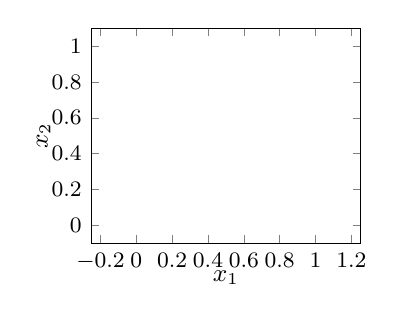
\begin{tikzpicture} 
\begin{axis}[view={\q}{20},axis equal,footnotesize,font=\footnotesize
  ,xlabel={$x_1$},ylabel={$x_2$},zlabel={$x_3$},label shift={-1.5ex} ]
    \threev[right]{2}{-1}{1}{\xv}
    \threev[right]{3.7}{-0.4}{2.3}{\xv'}
%    \threev[right]{1.2}{-1.3}{0.4}{\xv''}
%    \threev[right]{1.7}{-1.1}{0.8}{\xv'''}
\end{axis}
\end{tikzpicture}}
\end{center}


\item To explore further, let's say the second component of~\bv\ is in error by~1\% of~\bv, that is, by~\(0.1\).
As in the previous case, add \((0,0.1,0)\) to the right-hand side and solve to find now \(\xv''=(1.2,-1.3,0.4)\) which is quite different to both~\xv\ and~\(\xv'\), as illustrated below.
Compute its relative error \(|\xv-\xv''|/|\xv|=0.43\)\,.
At 43\%, the relative error in solution~\(\xv''\) is still much larger than the 1\%~error in~\bv.
\begin{center}
\qview{-52}{-48}{\begin{tikzpicture} 
\begin{axis}[view={\q}{20},axis equal,footnotesize,font=\footnotesize
  ,xlabel={$x_1$},ylabel={$x_2$},zlabel={$x_3$},label shift={-1.5ex} ]
    \threev[right]{2}{-1}{1}{\xv}
    \threev[right]{3.7}{-0.4}{2.3}{\xv'}
    \node[right] at (axis cs:1.2,-1.3,0.4) {$\xv''$};
    \addplot3[quiver={u=1.2,v=-1.3,w=0.4},blue,-stealth] coordinates {(0,0,0)};
    \node[right] at (axis cs:1.7,-1.1,0.8) {$\xv'''$};
    \addplot3[quiver={u=1.7,v=-1.1,w=0.8},blue,-stealth] coordinates {(0,0,0)};
\end{axis}
\end{tikzpicture}}
\end{center}

\item Lastly, let's say the third component of~\bv\ is in error by~1\% of~\bv, that is, by~\(0.1\).
As in the previous cases, add \((0,0,0.1)\) to the right-hand side and solve to find now \(\xv'''=(1.7,-1.1,0.8)\) which, as illustrated above, is at least is roughly~\xv.
Compute its relative error \(|\xv-\xv'''|/|\xv|=0.15\)\,.
At 15\%, the relative error in solution~\(\xv'''\) is still significantly larger than the 1\%~error in~\bv.

\end{enumerate}
This example shows that the apparently innocuous matrix~\(A\) variously multiples measurement errors in~\bv\ by factors of~\(91\), \(41\) or~\(15\) when finding `the solution'~\xv\ to \(A\xv=\bv\)\,.
The matrix~\(A\) must, after all, be a bad matrix.
Theorem~\ref{thm:erramp} shows this badness is quantified by its  condition number~\(152.27\), and its estimated reciprocal \verb|rcond|. 
\end{example}




\begin{example} \label{eg:} 
Consider solving the system of linear equations
\begin{equation*}
\begin{bmatrix} 0.4&0.4&-0.2&0.8
\\-0.2&0.8&-0.4&-0.4
\\0.4&-0.4&-0.8&-0.2
\\-0.8&-0.2&-0.4&0.4 \end{bmatrix}\xv
=\begin{bmatrix} -3\\3\\-9\\-1 \end{bmatrix}.
\end{equation*}
Use \script\ to explore the effect on the solution~\xv\ of 1\%~errors in the right-hand side vector.
\begin{solution} 
Enter the matrix and right-hand side vector into \script, then solve  with Procedure~\ref{pro:unisol}:
\setbox\ajrqrbox\hbox{\qrcode{% errors
Q=[0.4 0.4 -0.2 0.8
  -0.2 0.8 -0.4 -0.4
  0.4 -0.4 -0.8 -0.2
  -0.8 -0.2 -0.4 0.4]
b=[-3;3;-9;-1]
rcond(Q)
x=Q\slosh b
x1=Q\slosh(b+[0.1;0;0;0])
relerr1=norm(x-x1)/norm(x)
s=svd(Q)
condQ=s(1)/s(4)
}}%
\marginpar{\usebox{\ajrqrbox\\[2ex]}}%
\begin{verbatim}
Q=[0.4 0.4 -0.2 0.8
  -0.2 0.8 -0.4 -0.4
  0.4 -0.4 -0.8 -0.2
  -0.8 -0.2 -0.4 0.4]
b=[-3;3;-9;-1]
rcond(Q)
x=Q\b
\end{verbatim}
to find the solution \(\xv=(-4.6,5,7,-2.2)\).

Now see the effect on this solution of 1\%~errors in~\bv.
Since the length \(|\bv|=\verb|norm(b)|=10\) we find the solution for various changes to~\bv\ of size~\(0.1\).
\begin{itemize}
\item For example, adding the 1\%~error \((0.1,0,0,0)\) to~\bv, the \script\ commands
\begin{verbatim}
x1=Q\(b+[0.1;0;0;0])
relerr1=norm(x-x1)/norm(x)
\end{verbatim}
show the changed solution is \(\xv'=(-4.56,5.04,6.98,-2.12)\) which here is reasonably close to~\xv.
Indeed its relative error \(|\xv-\xv'|/|\xv|\) is computed to be~\(0.0100={}\)1\%.
Here the relative error in solution~\xv\ is exactly the same as the relative error in~\bv.

\item Exploring further, upon adding the 1\%~error \((0,0.1,0,0)\) to~\bv, analogous commands show the changed solution is \(\xv''=(-4.62,5.08,6.96,-2.24)\) which has relative error \(|\xv-\xv''|/|\xv|=0.0100={}\)1\% again.

\item Whereas, upon adding 1\%~error \((0,0,0.1,0)\) to~\bv, analogous commands show the changed solution is \(\xv'''=(-4.56,4.96,6.92,-2.22)\) which has relative error \(|\xv-\xv'''|/|\xv|=0.0100={}\)1\% again.

\item Lastly, upon adding 1\%~error \((0,0,0,0.1)\) to~\bv, analogous commands show the changed solution is \(\xv''''=(-4.68,4.98,6.96,-2.16)\) which has relative error \(|\xv-\xv''''|/|\xv|=0.0100={}\)1\% yet again.

\end{itemize}
In this example, and in contrast to the previous example, throughout the relative error in solution~\xv\ is exactly the same as the relative error in~\bv.
The reason is that here the matrix~\(Q\) is an \idx{orthogonal matrix}---check by computing \verb|Q'*Q| (Definition~\ref{def:orthog}).
Being orthogonal, multiplication by~\(Q\) only rotates or reflects, and so it never stretches or distorts (Theorem~\ref{thm:orthog:i}).
Consequently errors remain the same size when multiplied by such orthogonal matrices, as seen in this example, and as reflected in the condition number of~\(Q\) being one (as computed via \verb|s=svd(Q)| and then \verb|condQ=s(1)/s(4)|).
\end{solution}
\end{example}





The \idx{condition number} determines the reliability of the solution of a system of linear equations.
This is why we should always precede the computation of a solution with an estimate of the condition number such as that provided by the reciprocal~\verb|rcond()| (Procedure~\ref{pro:unisol}). 
The next theorem establishes that the condition number characterises the amplification of errors that occurs in solving a linear system.
Hence solving a system of linear equations with a large condition number (small \verb|rcond|) means that errors are amplified by a large factor as happens in Example~\ref{eg:ilsle}.

\begin{theorem}[error magnification] \label{thm:erramp}
Consider solving \(A\xv=\bv\) for \(n\times n\) matrix~\(A\) with full \(\rank A=n\)\,.  
\begin{aside}
The greek letter~\(\epsilon\) (epsilon) often denotes errors.
\end{aside}%
Suppose the right-hand side \bv~has relative error of size~\(\epsilon\), then the solution~\xv\ has relative error\({}\leq\epsilon\cond A\)\,, with equality in the worst case.
\end{theorem}

\begin{proof} 
Let the length of the right-hand side vector be \(b=|\bv|\).
Then the error in~\bv\ has size~\(\epsilon b\) since \(\epsilon\)~is the relative error.
Following Procedure~\ref{pro:gensol},
let \(A=\usv\) be an \svd\ for matrix~\(A\).
Compute \(\zv=\tr U\bv\)\,: recall that multiplication by orthogonal~\(U\) preserves lengths (Theorem~\ref{thm:orthog}), so not only is \(|\zv|=b\)\,, but also \zv~will be in error by an amount~\(\epsilon b\) since \bv~has this error 
Consider solving \(S\yv=\zv\)\,: the diagonals of~\(S\) stretch and shrink both `the signal and the noise'.
The \emph{worst case} is when \(\zv=(b,0,\ldots,0,\epsilon b)\); that is, when all the `signal' happens to be in the first component of~\zv, and all the `noise', the error, is in the last component.
Then the intermediary \(\yv=(b/\sigma_1,0,\ldots,\epsilon b/\sigma_n)\).
Consequently, the intermediary has relative error \((\epsilon b/\sigma_n)/(b/\sigma_1)=\epsilon(\sigma_1/\sigma_n)=\epsilon\cond A \)\,.
Again because multiplication by orthogonal~\(V\) preserves lengths, the solution \(\xv=V\yv\) has the same relative error:  in the worst case of~\(\epsilon\cond A\)\,.
\end{proof}

\begin{example} \label{eg:}
Each of the following cases involves solving a linear system \(A\xv=\bv\) to determine quantities of interest~\xv\ from some measured quantities~\bv.
From the given information estimate the maximum relative error in~\xv,  if  possible, otherwise say so.
\begin{enumerate}
\item Quantities~\bv\ are measured to a relative error~\(0.001\), and matrix~\(A\) has condition number of ten.
\item Quantities~\bv\ are measured to three significant digits and \(\verb|rcond(A)|=0.025\)\,.
\item Measurements are accurate to two decimal places, and matrix~\(A\) has condition number of twenty.
\item  Measurements are correct to two significant digits and \(\verb|rcond(A)|=0.002\)\,.
\end{enumerate}

\begin{solution} 
\begin{enumerate}
\item The relative error in~\xv\ could be as big as \(0.001\times10=0.01\)\,.
\item Measuring to three significant digits means the relative error is~\(0.0005\), while with \(\verb|rcond(A)|=0.025\)\,, matrix~\(A\) has condition number of roughly~\(40\), so the relative error of~\xv\ is less than \(0.0005\times40=0.02\)\,; that is, up to~2\%.
\item There is not enough information as we cannot determine the \emph{relative} error in measurements~\bv.
\item Two significant digits means the relative error is~\(0.005\), while matrix~\(A\) has condition number of roughly \(1/0.002=500\) so the relative error of~\xv\ could be as big as \(0.005\times500=2.5\)\,; that is, the estimate~\xv\ is possibly complete rubbish.
\end{enumerate}
\end{solution}
\end{example}




\begin{activity}
In some experiment the components of~\bv, \(|\bv|=5\)\,, are measured to two decimal places.
We compute a vector~\xv\ by solving \(A\xv=\bv\) with a matrix~\(A\) for which we compute \(\verb|rcond(A)|=0.02\)\,.
What is our estimate of the relative error in~\xv?
\partswidth=5em
\begin{parts}
\item 20\%
\item 5\% %%%%%%%%
\item 2\%
\item 0.1\%
\end{parts}
\end{activity}




This issue of the amplification of errors occurs in other contexts.
The eminent mathematician  \index{Poincar\'e, Henri}Henri Poincar\'e (1854--1912) was the first to detect possible chaos in the orbits of the planets.
\begin{quoted}{Poincar\'e, 1903}
If we knew exactly the laws of nature and the situation of the universe at the initial moment, we could predict exactly the situation of that same universe at a succeeding moment.
But even if it were the case that the natural laws had no longer any secret for us, we could still only know the initial situation approximately. 
If that enabled us to predict the succeeding situation with the same approximation, that is all we require, and we should say that the phenomenon had been predicted, that it is governed by laws. 
But it is not always so; it may happen that small differences in the initial conditions produce very great ones in the final phenomena. 
A small error in the former will produce an enormous error in the latter. 
Prediction becomes impossible, and we have the fortuitous phenomenon.
\end{quoted}
The analogue for us in solving linear equations such as \(A\xv=\bv\) is the following: it may happen that a small error in the elements of~\bv\ will produce an enormous error in the final~\xv.
The condition number warns when this happens by characterising the amplification. 



\index{condition number|)}




\subsection{Prove the SVD Theorem~\ref{thm:svd}}
\label{sec:psvdt}

% Maybe revise in light of the proof by Golub and van Loan p.70

\begin{quoted}{\index{Wiles, Andrew}Andrew Wiles, C1993}
When doing maths there's this great feeling.
You start with a problem that just mystifies you.
You can't understand it, it's so complicated, you just can't make head nor tail of it.
But then when you finally resolve it, you have this incredible feeling of how beautiful it is, how it all fits together so elegantly.
\end{quoted}


\begin{aside}
This proof may be delayed until the last week of a semester.
It may be given together with the closely related classic proof of Theorem~\ref{thm:smevec} on the eigenvectors of symmetric matrices.  
\end{aside}
Two preliminary examples introduce the structure of the general proof that an \svd\ exists.  
As in this example prelude, the proof of a general singular value decomposition is similarly constructive.

\subsubsection{Prelude to the proof}

These first two examples are optional: their purpose is to introduce key parts of the general proof in a definite setting.

\begin{example}[a \(2\times2\) case] \label{eg:2by2svdx}
Recall Example~\ref{eg:2by2svd} factorised the matrix
\begin{equation*}
A=\begin{bmatrix} 10&2\\5&11 \end{bmatrix}=
\begin{bmatrix} \frac35&-\frac45\\\frac45&\frac35 \end{bmatrix}
\begin{bmatrix} 10\sqrt2&0\\0&5\sqrt2 \end{bmatrix}
\tr{\begin{bmatrix} \frac1{\sqrt2}&-\frac1{\sqrt2}\\ \frac1{\sqrt2}&\frac1{\sqrt2} \end{bmatrix}}.
\end{equation*}
Find this factorisation, \(A=\usv\), by maximising~\(|A\vv|\) over all unit vectors~\vv.


\begin{solution} 
In 2D, all unit vectors are of the form \(\vv=(\cos t,\sin t)\) for \(-\pi<t\leq\pi\)\,.  
The marginal picture plots these unit vectors~\vv\ in blue for 32 angles~\(t\).
\marginpar{\eRose{10/10}{2/10}{5/10}{11/10}}%
\begin{aside}
The \script[1]\ function \texttt{eigshow(A)} provides an interactive alternative to this static view (click on the \texttt{eig/(svd)} button to make it show \texttt{svd/(eig)}.
\end{aside}%
Plotted in red from the end of each~\vv\ is the vector~\(A\vv\) (scaled down by a factor of ten for clarity).
Our aim is to find the~\vv\ that maximises the length of the corresponding adjoined~\(A\vv\).
By inspection, the longest red vectors~\(A\vv\) occur towards the top-right or the bottom-left, either of these directions~\vv\ are what we first find.

Maximising \(|A\vv|\) is the same as maximising~\(|A\vv|^2\) which is what the following considers: since
\begin{eqnarray*}
A\vv&=&\begin{bmatrix} 10&2\\5&11 \end{bmatrix}
\begin{bmatrix} \cos t\\\sin t \end{bmatrix}
=\begin{bmatrix} 10\cos t+2\sin t\\5\cos t+11\sin t \end{bmatrix},
\\|A\vv|^2&=&(10\cos t+2\sin t)^2+(5\cos t+11\sin t)^2
\\&=&100\cos^2 t+40\cos t\,\sin t+4\sin^2 t
\\&&{}+25\cos^2 t+110\cos t\,\sin t+121\sin^2 t
\\&=&125(\cos^2t+\sin^2t)+150\sin t\,\cos t
\\&=&125+75\sin 2t \qquad(\text{shown in the margin}).
\end{eqnarray*}
\marginpar{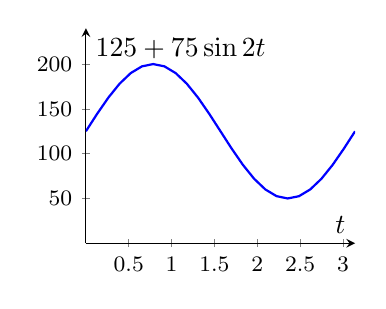
\begin{tikzpicture}
\begin{axis}[footnotesize,axis lines=middle
,xlabel={$t$},ylabel={$125+75\sin 2t$},ymin=0,ymax=240]
\addplot+[thick,no marks,domain=0:3.1415] {125+75*sin(deg(2*\x))};
\end{axis}
\end{tikzpicture}}%
Since the sine function has maximum of one at angle~\(\frac\pi2\), the maximum of~\(|A\vv|^2\) is~\(125+75=200\) for \(2t=\frac\pi2\)\,, that is, for \(t=\frac\pi4\) corresponding to unit vector \(\vv_1=(\cos\frac\pi4,\sin\frac\pi4)=(\frac1{\sqrt2},\frac1{\sqrt2})\)---this vector point to the top-right as identified from the marginal figure.
This vector is the first column of~\(V\).

Now multiply to find \(A\vv_1=(6\sqrt2,8\sqrt2)\).  
The length of this vector is \(\sqrt{72+128}=\sqrt{200}=10\sqrt 2=\sigma_1\) the leading singular value.  
Normalise the vector~\(A\vv_1\) by \(A\vv_1/\sigma_1 =(6\sqrt2,8\sqrt2)/(10\sqrt2) =(\frac35,\frac45) =\uv_1\)\,, the first column of~\(U\).

The other column of~\(V\) must be orthogonal (at right-angles) to~\(\vv_1\) in order for matrix~\(V\) to be orthogonal.
\marginpar{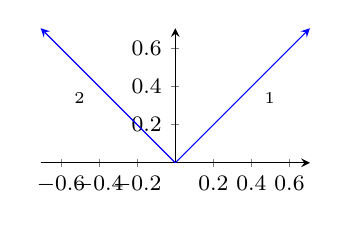
\begin{tikzpicture} 
\begin{axis}[axis equal image, axis lines=middle
,footnotesize,font=\footnotesize ]
    \addplot[quiver={u=0.707,v=0.707},blue,-stealth] 
    coordinates {(0,0)};
    \node at (axis cs:0.5,0.34) {$\vv_1$};
    \addplot[quiver={u=-0.707,v=0.707},blue,-stealth] 
    coordinates {(0,0)};
    \node at (axis cs:-0.5,0.34) {$\vv_2$};
\end{axis}
\end{tikzpicture}}%
Thus set \(\vv_2=(-\frac1{\sqrt2},\frac1{\sqrt2})\) as shown in the marginal graph.
Now multiply to find \(A\vv_2=(-4\sqrt2,3\sqrt2)\):
magically, and a crucial part of the general proof, this vector is orthogonal to~\(\uv_1\).
The length of \(A\vv_2=(-4\sqrt2,3\sqrt2)\) is \(\sqrt{32+18}=\sqrt{50}=5\sqrt2=\sigma_2\) the other singular value.
Normalise the vector to \(A\vv_2/\sigma_2 =(-4\sqrt2,3\sqrt2)/(2\sqrt2)=(-\frac45,\frac35)=\uv_2\)\,, the second column of~\(U\).

This construction establishes that here \(AV=US\)\,. 
Then post-multiply each side by~\(\tr V\) to find an \svd\ is \(A=\usv\).

In this example we could have chosen the negative of~\(\vv_1\) (angle \(t=-\frac{3\pi}4\)), and/or chosen the negative of~\(\vv_2\). 
The result would still be a valid \svd\ of the matrix~\(A\).
The orthogonal matrices in an \svd\ are not unique, and need not be. The singular values are unique.
\end{solution}
\end{example}

\begin{example}[a \(3\times1\) case] \label{eg:3x1svd}
\def\thr{\frac1{\sqrt 3}}
Find the following \svd\ for the \(3\times1\) matrix
\begin{equation*}
A=\begin{bmatrix} 1\\1\\1 \end{bmatrix}
=\begin{bmatrix} \thr&\cdot&\cdot\;
\\\thr&\cdot&\cdot
\\\thr&\cdot&\cdot \end{bmatrix}
\begin{bmatrix} \sqrt3\\0\\0 \end{bmatrix}
\tr{\begin{bmatrix} 1 \end{bmatrix}}=\usv,
\end{equation*}
where we do not worry about the elements denoted by dots as they are multiplied by the zeros in~\(S=(\sqrt3,0,0)\).
\begin{solution} 
We seek to maximise \(|A\vv|^2\) but here vector~\vv\ is in~\(\RR^1\).  
Being of unit magnitude, there are two alternatives: \(\vv=(\pm 1)\). 
Each alternative gives the same \(|A\vv|^2=|(\pm1,\pm1,\pm1)|=3\)\,.  
Choose one alternative, say \(\vv_1=(1)\), fixes the matrix \(V=\begin{bmatrix} 1 \end{bmatrix}\).

Then \(A\vv_1=(1,1,1)\) which is of length~\(\sqrt3\).
This length is the singular value \(\sigma_1=\sqrt3\)\,.  
Dividing~\(A\vv_1\) by its length gives the unit vector \(\uv_1=(\thr,\thr,\thr)\), the first column of~\(U\).  
To find the other columns of~\(U\), consider the three standard unit vectors in~\(\RR^3\) (red in the illustration below), rotate them all together so that one lines up with~\(\uv_1\), and then the other two rotated unit vectors form the other two columns of~\(U\) (blue vectors below).  
Since the columns of~\(U\) are then orthonormal, \(U\)~is an orthogonal matrix (Theorem~\ref{thm:orthog}).
\end{solution}
\begin{center}
\qview{55}{60}{\begin{tikzpicture} 
\begin{axis}[axis equal image,footnotesize,font=\footnotesize,view={\q}{20}]
    \addplot3[quiver={u=1,v=0,w=0},red,-stealth] coordinates {(0,0,0)};
    \addplot3[quiver={u=0,v=1,w=0},red,-stealth] coordinates {(0,0,0)};
    \addplot3[quiver={u=0,v=0,w=1},red,-stealth] coordinates {(0,0,0)};
    \node[left] at (axis cs:1,0,0) {$\vec e_1$};
    \node[below] at (axis cs:0,1,0) {$\vec e_2$};
    \node[right] at (axis cs:0,0,1) {$\vec e_3$};
\threev[above]{0.58}{0.58}{0.58}{\vec u_1}
\threev{0.58}{-0.79}{0.21}{};
\threev{-0.58}{-0.21}{0.79}{};
\end{axis}
\end{tikzpicture}}
\end{center}
\end{example}





\paragraph{Outline of the general proof} 
We use \idx{induction} 
\ifcsname r@sec:pi\endcsname (section~\ref{sec:pi}) \fi
on the size \(m\times n\) of the matrix.
\begin{itemize}
\item First zero matrices have trivial \svd, and
\(m\times 1\) and \(1\times n\) matrices have straightforward \svd\ (as in Example~\ref{eg:3x1svd}).
\item Choose \(\vv_1\) to maximise~\(|A\vv|^2\) for unit vectors \(\vv\) in~\(\RR^n\).
\item Crucially, we then establish that for every vector~\vv\ orthogonal to~\(\vv_1\), the vector \(A\vv\) is orthogonal to~\(A\vv_1\).
\item Then rotate the standard unit vectors to align one with~\(\vv_1\). Similarly for~\(A\vv_1\).  
\item This rotation transforms the matrix~\(A\) to strip off the leading singular value, and effectively leave an \((m-1)\times(n-1)\) matrix.
\item  By induction on the size, an \svd\ exists for all sizes.
\end{itemize}
This proof corresponds closely to the proof of the spectral theorem~\ref{thm:smevec} for symmetric matrices of section~\ref{sec:sm}. 





\subsubsection{Detailed proof of the SVD Theorem~\ref{thm:svd}}
\label{sec:dpsvdt}

Use \idx{induction} on the size \(m\times n\) of the matrix~\(A\): we assume an \svd\ exists for all \((m-1)\times(n-1)\)~matrices, and prove that consequently an \svd\ must exist for all \(m\times n\)~matrices.  There are three base cases to establish: one for \(m\leq n\)\,, one for \(m\geq n\)\,, and one for matrix \(A=O\)\,; then the induction extends to all sized matrices.

\paragraph{Case $A=O_{m\times n}$:}
When \(m\times n\) matrix \(A=O_{m\times n}\) then choose \(U=I_m\) (orthogonal), \(S=O_{m\times n}\) (diagonal), and \(V=I_n\) (orthogonal) so then \(\usv=I_mO_{m\times n}\tr I_n=O_{m\times n}=A\)\,.  

Consequently, the rest of the proof only considers the non-trivial cases when the matrix~\(A\) is not all zero. 



\paragraph{Case $m\times 1$ ($n=1$):}
Here the \(m\times 1\) nonzero matrix \(A=\begin{bmatrix} \av_1 \end{bmatrix}\) for \(\av_1=(a_{11},a_{21},\ldots,a_{m1})\).
%%%% So far avoided using $\sum$ at all
%Set \(\sigma_1=|\av_1|=\sqrt{\sum_i a_{i1}^2}\) and unit vector \(\uv_1=\av_1/\sigma_1\).
Set the singular value \(\sigma_1=|\av_1|=\sqrt{a_{11}^2+a_{21}^2+\cdots+a_{m1}^2}\) and unit vector \(\uv_1=\av_1/\sigma_1\).
Set \(1\times 1\) orthogonal matrix \(V=\begin{bmatrix} 1 \end{bmatrix}\);
\(m\times 1\) diagonal matrix 
%\(S=\begin{bmatrix} \sigma_1\\0\\\vdots\\0 \end{bmatrix}\); and
\(S=(\sigma_1,0,\ldots,0)\); and
\(m\times m\) orthogonal matrix \(U=\begin{bmatrix} \uv_1 &\uv_2&\cdots&\uv_m\end{bmatrix}\).
Matrix~\(U\) exists because we can take the orthonormal set of standard unit vectors in~\(\RR^m\) and rotate them all together so that the first lines up with~\(\uv_1\): the other \((m-1)\)~unit vectors then become the other~\(\uv_j\).
Then an \svd\ for the \(m\times1\) matrix~\(A\) is
\begin{eqnarray*}
\usv
&=&\begin{bmatrix} \uv_1 &\uv_2&\cdots&\uv_m\end{bmatrix}
\begin{bmatrix} \sigma_1\\0\\\vdots\\0 \end{bmatrix}
\tr{1}
\\&=&\sigma_1{\uv_1}
=\begin{bmatrix} \av_1 \end{bmatrix}
=A\,.
\end{eqnarray*}

\paragraph{Case $1\times n$ ($m=1$):}
use an exactly complementary argument to the preceding \(m\times1\) case.
%Here \(1\times n\) nonzero matrix \(A=\begin{bmatrix} a_{1j} \end{bmatrix}\).
%Set \(\sigma_1=\sqrt{\sum_j a_{1j}^2}\) and unit vector \(\vv_1=(a_{1i})/\sigma_1\).
%Set \(1\times 1\) orthogonal matrix \(U=\begin{bmatrix} 1 \end{bmatrix}\);
%\(1\times n\) `diagonal' matrix \(S=\begin{bmatrix} \sigma_1&0&\cdots&0 \end{bmatrix}\); and
%\(n\times n\) orthogonal matrix \(V=\begin{bmatrix} \vv_1 &\vv_2&\cdots&\vv_n\end{bmatrix}\).
%Matrix~\(V\) exists because we can take the orthonormal set of standard unit vectors in~\(\RR^n\) and rotate them all together so that the first lines up with~\(\vv_1\): the other \((n-1)\)~unit vectors then become the other~\(\vv_j\).
%Then 
%\(\usv
%=1\begin{bmatrix} \sigma_1&0&\cdots&0 \end{bmatrix}
%\tr{\begin{bmatrix} \vv_1 &\vv_2&\cdots&\vv_n\end{bmatrix}}
%=\sigma_1\tr{\vv_1}
%=\begin{bmatrix} a_{1j} \end{bmatrix}
%=A
%\)



\paragraph{Induction}  
Assume  an \svd\ exists for all \((m-1)\times(n-1)\)~matrices: we proceed to prove that consequently an \svd\ must exist for all \(m\times n\)~matrices.
Consider any \(m\times n\) nonzero matrix~\(A\) for \(m,n\geq2\)\,.
Set vector~\(\vv_1\) in~\(\RR^n\) to be a \emph{unit vector} that maximises~\(|A\vv|^2\) for unit vectors \(\vv\) in~\(\RR^n\); that is, vector~\(\vv_1\) achieves the \idx{maximum} in \(\max_{|\vv|=1}|A\vv|^2\).
\begin{enumerate}
\item \emph{Such a maximum exists by the Extreme Value Theorem in Calculus.}
Proved in higher level analysis.

%Optional (omit as no real need): confirm that a maximum exists by bounding it.
%Let \(\uv:=A\vv\) so \(u_i=\sum_{n=1}^na_{ij}v_j\)\,.
%Then, upon setting \(a:=\max_{i,j}|a_{ij}|\) and using \(|v_j|\leq1\) as \(|\vv|=1\)\,,
%\begin{equation*}
%|u_i|\leq\sum_{n=1}^n|a_{ij}||v_j|
%\leq\sum_{n=1}^na\cdot1
%=na\,.
%\end{equation*}
%Consequently,
%\begin{equation*}
%|A\vv|^2=|\uv|^2=\sum_{i=1}^m u_i^2
%\leq\sum_{i=1}^m (na)^2 = mn^2a^2.
%\end{equation*}
%Such a bound corresponds to the existence of a maximum of~\(|A\vv|^2\): out of all the any unit vectors that achieve the maximum value, choose any one to be~\(\vv_1\).
%
As matrix~\(A\) is nonzero, there exists~\vv\ such that \(|A\vv|>0\)\,.
Since \(\vv_1\) maximises \(|A\vv|\) it follows that \(|A\vv_1|>0\)\,.
%Observe that \(|A\vv_1|>0\) as matrix~\(A\) is nonzero.
%Let \(i^*,j^*\) achieve the maximum \(a:=\max_{i,j}|a_{ij}|\)\,: \(a>0\) as the matrix is not all zero. 
%Choosing the unit vector~\(\vv\) to be zero except for a one in the \(j^*\)th~position, the maximum \(|A\vv_1|\geq|A\vv|=|\av_{j^*}|\geq a>0\)\,.

\emph{The vector~\(\vv_1\) is not unique:} for example, the negative~\(-\vv_1\) is another unit vector that achieves the maximum value.  
Sometimes there are other unit vectors that achieve the maximum value. 
Choose any one of them. 

Nonetheless, the maximum value of~\(|A\vv|^2\) is unique, and so the following singular value~\(\sigma_1\) is unique.

\item \emph{Set the singular value \(\sigma_1:=|A\vv_1|>0\) and unit vector \(\uv_1:=(A\vv_1)/\sigma_1\) in~\(\RR^m\). 
Let~\vv\ be any unit vector orthogonal to~\(\vv_1\): we prove that then the vector~\(A\vv\) is orthogonal to~\(\uv_1\).}
Let \(\uv:=A\vv\) in~\(\RR^m\) and consider \(f(t):=|A(\vv_1\cos t+\vv\sin t)|^2\).
Since \(\vv_1\) achieves the maximum, and \(\vv_1\cos t+\vv\sin t\) is a unit vector for all~\(t\) (Exercise~\ref{ex:univec}), then \(f(t)\)~must have a maximum at \(t=0\) (maybe at other~\(t\) as well), and so \(f'(0)=0\) (from the Calculus of a maximum).
On the other hand, 
\begin{eqnarray*}
f(t)&=&|A\vv_1\cos t+A\vv\sin t|^2
\\&=&|\sigma_1\uv_1\cos t+\uv\sin t|^2
\\&=&(\sigma_1\uv_1\cos t+\uv\sin t)\cdot(\sigma_1\uv_1\cos t+\uv\sin t)
\\&=&\sigma_1^2\cos^2 t+\sigma_1\uv\cdot\uv_12\sin t\,\cos t+|\uv|^2\sin^2 t
\,;
\end{eqnarray*}
differentiating~\(f(t)\) and evaluating at zero gives
\(f'(0)=\sigma_1\uv\cdot\uv_1\)\,.
But from the maximum this derivative is zero, so \(\sigma_1\uv\cdot\uv_1=0\)\,.
Since the singular value \(\sigma_1>0\)\,, we must have \(\uv\cdot\uv_1=0\) and so \(\uv_1\) and~\(\uv\) are orthogonal (Definition~\ref{def:orthovec}).

\item Consider the orthonormal set of standard unit vectors in~\(\RR^n\): rotate them so that the first unit vector lines up with~\(\vv_1\), and let the other \((n-1)\)~rotated unit vectors become the columns of the \(n\times(n-1)\) matrix~\(\bar V\).
Then set the \(n\times n\) matrix
\(V_1:=\begin{bmatrix}\vv_1&\bar V\end{bmatrix}\) which is orthogonal as its columns are orthonormal (Theorem~\ref{thm:orthog:ii}).
Similarly set an \(m\times m\) orthogonal matrix
\(U_1:=\begin{bmatrix}\uv_1&\bar U\end{bmatrix}\).
Compute the \(m\times n\) matrix
\begin{eqnarray*}
A_1:=\tr{U_1}AV_1
&=&\begin{bmatrix} \tr{\uv_1}\\\tr{\bar U} \end{bmatrix}A
\begin{bmatrix} \vv_1 &\bar V \end{bmatrix}
\\&=&\begin{bmatrix} \tr{\uv_1}A\vv_1 & \tr{\uv_1}A\bar V
\\\tr{\bar U}A\vv_1&\tr{\bar U}A\bar V \end{bmatrix}
\end{eqnarray*}
where
\begin{itemize}
\item the top-left entry \(\tr{\uv_1}A\vv_1=\tr{\uv_1}\sigma_1\uv_1=\sigma_1|\uv_1|^2=\sigma_1\)\,,
\item the bottom-left column \(\tr{\bar U}A\vv_1=\tr{\bar U}\sigma_1\uv_1=O_{m-1\times 1}\) as the columns of~\(\bar U\) are orthogonal to~\(\uv_1\),
\item the top-right row \(\tr{\uv_1}A\bar V=O_{1\times n-1}\) as each column of~\(\bar V\) is orthogonal to~\(\vv_1\) and hence each column of~\(A\bar V\) is orthogonal to~\(\uv_1\),
\item and set the bottom-right block \(B:=\tr{\bar U}A\bar V\) which is an \((m-1)\times(n-1)\) matrix as \(\tr{\bar U}\) is~\((m-1)\times m\) and \(\bar V\) is \(n\times(n-1)\).
\end{itemize}
Consequently, 
\begin{equation*}
A_1=\begin{bmatrix} \sigma_1&O_{1\times n-1}
\\O_{m-1\times 1}&B \end{bmatrix}.
\end{equation*}%
Note: rearranging \(A_1:=\tr{U_1}AV_1\) gives \(AV_1=U_1A_1\).

\item \emph{By induction assumption, \((m-1)\times(n-1)\) matrix~\(B\) has an \svd, and so we now construct an \svd\ for \(m\times n\) matrix~\(A\).}
Let \(B=\hat U\hat S\tr{\hat V}\) be an \svd\ for~\(B\).
Then construct 
%\begin{equation*}
%U:=U_1\begin{bmatrix} 1&O_{1\times m-1}\\O_{m-1\times 1}&\hat U \end{bmatrix},\quad
%V:=\begin{bmatrix} 1&O_{1\times n-1}\\O_{n-1\times 1}&\hat V\end{bmatrix}V_1,\quad
%S:=\begin{bmatrix} \sigma_1&O_{1\times n-1}\\O_{m-1\times 1}&\hat S \end{bmatrix}.
%\end{equation*}
\begin{equation*}
U:=U_1\begin{bmatrix} 1&0\\0&\hat U \end{bmatrix},\quad
V:=V_1\begin{bmatrix} 1&0\\0&\hat V\end{bmatrix},\quad
S:=\begin{bmatrix} \sigma_1&0\\0&\hat S \end{bmatrix}.
\end{equation*}
Matrices \(U\) and~\(V\) are orthogonal as each are the product of two orthogonal matrices (Exercise~\ref{ex:orthoprod}), and matrix~\(S\) is diagonal.
These form an \svd\ for matrix~\(A\) since
\begin{eqnarray*}
AV&=&AV_1\begin{bmatrix} 1&0\\0&\hat V\end{bmatrix}
=U_1A_1\begin{bmatrix} 1&0\\0&\hat V\end{bmatrix}
\\&=&U_1\begin{bmatrix} \sigma_1&0 \\0&B \end{bmatrix}\begin{bmatrix} 1&0\\0&\hat V\end{bmatrix}
=U_1\begin{bmatrix} \sigma_1&0 \\0&B\hat V \end{bmatrix}
\\&=&U_1\begin{bmatrix} \sigma_1&0 \\0&\hat U\hat S \end{bmatrix}
=U_1\begin{bmatrix} 1&0 \\0&\hat U \end{bmatrix}
\begin{bmatrix} \sigma_1&0 \\0&\hat S \end{bmatrix}
\\&=&US.
\end{eqnarray*}
Hence \(A=\usv\). 
By induction, an \svd\ exists for all \(m\times n\) matrices.
\end{enumerate}
This argument establishes the \svd\ Theorem~\ref{thm:svd}.







\subsection{Exercises}



\begin{exercise} \label{ex:} 
Using a factorisation of the left-hand side coefficient, quickly solve by hand the following equations.
% p=[2,3,5,7,11]; c=prod(p(ceil(5*rand(1,3)))),b=c*ceil(40+60*rand)
\begin{parts}
\item \(18 x=1134\)
\item \(42 x=2226\)
\item \(66 x=3234\)
\item \(70 x=3150\)
\item \(99 x=8118\)
\item \(154 x=7854\)
\item \(175 x=14350\)
\item \(242 x=20086\)
\item \(245 x=12495\)
\item \(363 x=25047\)
\item \(385 x=15785\)
\item \(539 x=28028\)
\end{parts}
\end{exercise}




\begin{exercise} \label{ex:hsledvs} 
Find a general solution, if a solution exists, of each of the following systems of \idx{linear equation}s using Procedure~\ref{pro:gensol}.
Calculate by hand using the given \svd\ factorisation; record your working.
% Change any part of this exercise => change a later question.
% u=randq(m), s=diag(-sort(-round(abs(randn(1,4).^2))/2),m,n), v=randq(n), x=v*s'*round(randn(m,1)*4)/2, A=u*s*v', b=A*x
\begin{enumerate}
\item \(\underbrace{\begin{bmatrix} -\frac{9}{5}&\frac{12}{5}
\\-4&-3 \end{bmatrix}}_{=\eAii}\xv
=\begin{bmatrix} -\frac{9}{5}
\\\frac{17}{2} \end{bmatrix}\) given the \svd
\begin{equation*}
\eAii=\begin{bmatrix} 0&1
\\1&0 \end{bmatrix}
\begin{bmatrix} 5&0
\\0&3 \end{bmatrix}
\tr{\begin{bmatrix} -\frac{4}{5}&-\frac{3}{5}
\\-\frac{3}{5}&\frac{4}{5} \end{bmatrix}}
\end{equation*}
\answer{\(\xv=(-1,-\frac{3}{2})\)}

\item \(\underbrace{\begin{bmatrix} \frac{15}{13}&\frac{36}{13}
\\\frac{36}{13}&-\frac{15}{13} \end{bmatrix}}_{=\eAii}\xv
=\begin{bmatrix} \frac{54}{13}
\\-\frac{45}{26} \end{bmatrix}\) given the \svd
\begin{equation*}
\eAii=\begin{bmatrix} -\frac{12}{13}&\frac{5}{13}
\\\frac{5}{13}&\frac{12}{13} \end{bmatrix}
\begin{bmatrix} 3&0
\\0&3 \end{bmatrix}
\tr{\begin{bmatrix} 0&1
\\-1&0 \end{bmatrix}}
\end{equation*}
\answer{\(\xv=(0,\frac{3}{2})\)}

\item \(\underbrace{\begin{bmatrix} -0.96&1.28
\\-0.72&0.96 \end{bmatrix}}_{=\eAii}\xv
=\begin{bmatrix} 2.88
\\2.16 \end{bmatrix}\) given the \svd
\begin{equation*}
\eAii=\begin{bmatrix} \frac{4}{5}&\frac{3}{5}
\\\frac{3}{5}&-\frac{4}{5} \end{bmatrix}
\begin{bmatrix} 2&0
\\0&0 \end{bmatrix}
\tr{\begin{bmatrix} -\frac{3}{5}&-\frac{4}{5}
\\\frac{4}{5}&-\frac{3}{5} \end{bmatrix}}
\end{equation*}
\answer{\(\xv=(-1.08,1.44)-(0.8,0.6)t\)}

\item \(\underbrace{\begin{bmatrix} -\frac{5}{26}&-\frac{6}{13}
\\-\frac{12}{13}&\frac{5}{13} \end{bmatrix}}_{=\eAii}\xv
=\begin{bmatrix} -\frac{7}{13}
\\\frac{34}{13} \end{bmatrix}\) given the \svd
\begin{equation*}
\eAii=\begin{bmatrix} 0&1
\\1&0 \end{bmatrix}
\begin{bmatrix} 1&0
\\0&\frac{1}{2} \end{bmatrix}
\tr{\begin{bmatrix} -\frac{12}{13}&-\frac{5}{13}
\\\frac{5}{13}&-\frac{12}{13} \end{bmatrix}}
\end{equation*}
\answer{\(\xv=(-2,2)\)}

\item \(\underbrace{\begin{bmatrix} -\frac{2}{3}&\frac{23}{51}&\frac{22}{51}
\\\frac{1}{6}&\frac{7}{51}&-\frac{31}{51} \end{bmatrix}}_{=\eAii}\xv
=\begin{bmatrix} -\frac{115}{102}
\\-\frac{35}{102} \end{bmatrix}\) given the \svd
\begin{equation*}
\eAii=\begin{bmatrix} \frac{15}{17}&-\frac{8}{17}
\\-\frac{8}{17}&-\frac{15}{17} \end{bmatrix}
\begin{bmatrix} 1&0&0
\\0&\frac{1}{2}&0 \end{bmatrix}
\tr{\begin{bmatrix} -\frac{2}{3}&\frac{1}{3}&-\frac{2}{3}
\\\frac{1}{3}&-\frac{2}{3}&-\frac{2}{3}
\\\frac{2}{3}&\frac{2}{3}&-\frac{1}{3} \end{bmatrix}}
\end{equation*}
\answer{\(\xv=(\frac{10}{9},-\frac{25}{18},\frac{5}{9})-(\frac{2}{3},\frac{2}{3},\frac{1}{3})t\)}

\item \(\underbrace{\begin{bmatrix} \frac{3}{35}&\frac{9}{35}&\frac{9}{70}
\\-\frac{4}{35}&-\frac{12}{35}&-\frac{6}{35} \end{bmatrix}}_{=\eAii}\xv
=\begin{bmatrix} \frac{3}{8}
\\-\frac{1}{2} \end{bmatrix}\) given the \svd
\begin{equation*}
\eAii=\begin{bmatrix} -\frac{3}{5}&\frac{4}{5}
\\\frac{4}{5}&\frac{3}{5} \end{bmatrix}
\begin{bmatrix} \frac{1}{2}&0&0
\\0&0&0 \end{bmatrix}
\tr{\begin{bmatrix} -\frac{2}{7}&-\frac{6}{7}&\frac{3}{7}
\\-\frac{6}{7}&\frac{3}{7}&\frac{2}{7}
\\-\frac{3}{7}&-\frac{2}{7}&-\frac{6}{7} \end{bmatrix}}
\end{equation*}
\answer{\(\xv=(\frac{5}{14},\frac{15}{14},\frac{15}{28})
+(-\frac{6}{7},\frac{3}{7},-\frac{2}{7})s
+(\frac{3}{7},\frac{2}{7},-\frac{6}{7})t\)}

\item \(\underbrace{\begin{bmatrix} \frac{7}{39}&-\frac{17}{39}
\\-\frac{22}{39}&-\frac{19}{39}
\\-\frac{4}{39}&-\frac{53}{78} \end{bmatrix}}_{=\eAii}\xv
=\begin{bmatrix} -\frac{1}{3}
\\-\frac{2}{3}
\\-\frac{2}{3} \end{bmatrix}\) given the \svd
\begin{equation*}
\eAii=\begin{bmatrix} -\frac{1}{3}&\frac{2}{3}&\frac{2}{3}
\\-\frac{2}{3}&-\frac{2}{3}&\frac{1}{3}
\\-\frac{2}{3}&\frac{1}{3}&-\frac{2}{3} \end{bmatrix}
\begin{bmatrix} 1&0
\\0&\frac{1}{2}
\\0&0 \end{bmatrix}
\tr{\begin{bmatrix}&\frac{5}{13}&\frac{12}{13}
\\\frac{12}{13}&-\frac{5}{13} \end{bmatrix}}
\end{equation*}
\answer{\(\xv=(\frac{5}{13},\frac{12}{13})\)}


\item \(\underbrace{\begin{bmatrix} \frac{36}{119}&-\frac{11}{17}
\\\frac{164}{119}&-\frac{18}{17}
\\-\frac{138}{119}&-\frac{6}{17} \end{bmatrix}}_{=\eAii}\xv
=\begin{bmatrix} \frac{11}{17}
\\\frac{9}{17}
\\\frac{3}{17} \end{bmatrix}\) given the \svd
\begin{equation*}
\eAii=\begin{bmatrix} \frac{2}{7}&-\frac{3}{7}&-\frac{6}{7}
\\\frac{6}{7}&-\frac{2}{7}&\frac{3}{7}
\\-\frac{3}{7}&-\frac{6}{7}&\frac{2}{7} \end{bmatrix}
\begin{bmatrix} 2&0
\\0&1
\\0&0 \end{bmatrix}
\tr{\begin{bmatrix} \frac{15}{17}&\frac{8}{17}
\\-\frac{8}{17}&\frac{15}{17} \end{bmatrix}}
\end{equation*}
\answer{No solution.}

\item \(\underbrace{\begin{bmatrix} -\frac{17}{18}&-\frac{8}{9}&-\frac{8}{9}
\\1&\frac{2}{3}&-\frac{2}{3}
\\-\frac{11}{9}&\frac{8}{9}&-\frac{7}{9} \end{bmatrix}}_{=\eAii}\xv
=\begin{bmatrix} -\frac{17}{18}
\\\frac{5}{3}
\\-\frac{7}{18} \end{bmatrix}\) given the \svd
\begin{equation*}
\eAii=\begin{bmatrix} -\frac{2}{3}&-\frac{1}{3}&-\frac{2}{3}
\\\frac{1}{3}&\frac{2}{3}&-\frac{2}{3}
\\-\frac{2}{3}&\frac{2}{3}&\frac{1}{3} \end{bmatrix}
\begin{bmatrix} 2&0&0
\\0&\frac{3}{2}&0
\\0&0&1 \end{bmatrix}
\tr{\begin{bmatrix} \frac{8}{9}&\frac{1}{9}&-\frac{4}{9}
\\\frac{1}{9}&\frac{8}{9}&\frac{4}{9}
\\\frac{4}{9}&-\frac{4}{9}&\frac{7}{9} \end{bmatrix}}
\end{equation*}
\answer{\(\xv=(1,\frac{1}{2},-\frac{1}{2})\)}

\item \(\underbrace{\begin{bmatrix} -\frac{10}{27}&-\frac{2}{27}&\frac{31}{54}
\\-\frac{4}{27}&\frac{10}{27}&\frac{17}{27}
\\-\frac{8}{27}&-\frac{7}{27}&\frac{7}{27} \end{bmatrix}}_{=\eAii}\xv
=\begin{bmatrix} \frac{83}{54}
\\\frac{49}{54}
\\\frac{17}{54} \end{bmatrix}\) given the \svd
\begin{equation*}
\eAii=\begin{bmatrix} -\frac{2}{3}&\frac{1}{3}&-\frac{2}{3}
\\-\frac{2}{3}&-\frac{2}{3}&\frac{1}{3}
\\-\frac{1}{3}&\frac{2}{3}&\frac{2}{3} \end{bmatrix}
\begin{bmatrix} 1&0&0
\\0&\frac{1}{2}&0
\\0&0&0 \end{bmatrix}
\tr{\begin{bmatrix} \frac{4}{9}&-\frac{4}{9}&\frac{7}{9}
\\-\frac{1}{9}&-\frac{8}{9}&-\frac{4}{9}
\\-\frac{8}{9}&-\frac{1}{9}&\frac{4}{9} \end{bmatrix}}
\end{equation*}
\answer{No solution.}

\item \(\underbrace{\begin{bmatrix} \frac{4}{33}&\frac{4}{11}&\frac{6}{11}
\\\frac{4}{33}&\frac{4}{11}&\frac{6}{11}
\\\frac{2}{33}&\frac{2}{11}&\frac{3}{11} \end{bmatrix}}_{=\eAii}\xv
=\begin{bmatrix} -\frac{7}{3}
\\-\frac{7}{3}
\\-\frac{7}{6} \end{bmatrix}\) given the \svd
\begin{equation*}
\eAii=\begin{bmatrix} \frac{2}{3}&-\frac{2}{3}&\frac{1}{3}
\\\frac{2}{3}&\frac{1}{3}&-\frac{2}{3}
\\\frac{1}{3}&\frac{2}{3}&\frac{2}{3} \end{bmatrix}
\begin{bmatrix} 1&0&0
\\0&0&0
\\0&0&0 \end{bmatrix}
\tr{\begin{bmatrix} \frac{2}{11}&-\frac{9}{11}&\frac{6}{11}
\\\frac{6}{11}&\frac{6}{11}&\frac{7}{11}
\\\frac{9}{11}&-\frac{2}{11}&-\frac{6}{11} \end{bmatrix}}
\end{equation*}
\answer{\(\xv=(-\frac{7}{11},-\frac{21}{11},-\frac{63}{22})+(-\frac{9}{11}.\frac{6}{11},-\frac{2}{11})s+(\frac{6}{11},\frac{7}{11},-\frac{6}{11})t\)}

\item \(\underbrace{\begin{bmatrix} -\frac{6}{11}&-\frac{1}{11}&\frac{81}{22}
\\\frac{7}{11}&\frac{3}{11}&\frac{27}{11}
\\-\frac{6}{11}&\frac{9}{22}&-\frac{9}{11} \end{bmatrix}}_{=\eAii}\xv
=\begin{bmatrix} -\frac{35}{2}
\\-\frac{41}{4}
\\\frac{15}{8} \end{bmatrix}\) given the \svd
\begin{equation*}
\eAii=\begin{bmatrix} \frac{9}{11}&\frac{6}{11}&\frac{2}{11}
\\\frac{6}{11}&-\frac{7}{11}&-\frac{6}{11}
\\-\frac{2}{11}&\frac{6}{11}&-\frac{9}{11} \end{bmatrix}
\begin{bmatrix} \frac{9}{2}&0&0
\\0&1&0
\\0&0&\frac{1}{2} \end{bmatrix}
\tr{\begin{bmatrix} 0&-1&0
\\0&0&-1
\\1&0&0 \end{bmatrix}}
\end{equation*}
\answer{\(\xv=(2,-\frac{7}{4},-\frac{9}{2})\)}


\end{enumerate}
\end{exercise}



\begin{exercise} \label{ex:csledvs} 
Find a general solution, if a solution exists, of each of the following systems of linear equations.
Calculate by hand using the given \svd\ factorisation; check the \svd\ and confirm your calculations with \script\ (Procedure~\ref{pro:gensol}); then compare and contrast the two methods.
% Change any part of this exercise => change a later exercise.
% u=randq(m), s=diag(-sort(-round(abs(randn(1,4)*2))),m,n), v=randq(n), x=v*s'*round(randn(m,1)*4), A=u*s*v', b=A*x

\arraycolsep=0.2em % gives room for QR-code??
\begin{enumerate}
\item \(\underbrace{\begin{bmatrix} \frac{7}{180}&\frac{8}{45}&\frac{41}{180}
\\\frac{19}{180}&-\frac{22}{45}&\frac{101}{180}
\\-\frac{19}{180}&\frac{4}{45}&\frac{133}{180}
\\\frac{59}{60}&-\frac{2}{15}&\frac{91}{60} \end{bmatrix}}_{=\eAii}\xv
=\begin{bmatrix} -\frac{13}{40}
\\-\frac{9}{8}
\\-\frac{17}{20}
\\-\frac{15}{4} \end{bmatrix}\) given the \svd
\setbox\ajrqrbox\hbox{\qrcode{% SVD
U=[-1 3 3 -9
-3 -9 -1 -3
-3 -1 9 3
-9 3 -3 1]/10
S=[2 0 0
0 1/2 0
0 0 1/2
0 0 0]
V=[-4 4 -7
1 8 4
-8 -1 4]/9
}}%
\marginpar{\usebox{\ajrqrbox\\[2ex]}}%
\begin{equation*}
\eAii=\begin{bmatrix} -\frac{1}{10}&\frac{3}{10}&\frac{3}{10}&-\frac{9}{10}
\\-\frac{3}{10}&-\frac{9}{10}&-\frac{1}{10}&-\frac{3}{10}
\\-\frac{3}{10}&-\frac{1}{10}&\frac{9}{10}&\frac{3}{10}
\\-\frac{9}{10}&\frac{3}{10}&-\frac{3}{10}&\frac{1}{10} \end{bmatrix}
\begin{bmatrix} 2&0&0
\\0&\frac{1}{2}&0
\\0&0&\frac{1}{2}
\\0&0&0 \end{bmatrix}
\tr{\begin{bmatrix} -\frac{4}{9}&\frac{4}{9}&-\frac{7}{9}
\\\frac{1}{9}&\frac{8}{9}&\frac{4}{9}
\\-\frac{8}{9}&-\frac{1}{9}&\frac{4}{9} \end{bmatrix}}
\end{equation*}
\answer{\(\xv=(-\frac{19}{12},\frac{1}{3},-\frac{17}{12})\)}


\item \(\underbrace{\begin{bmatrix} \frac{79}{66}&\frac{7}{33}&-\frac{29}{33}
\\-\frac{65}{66}&-\frac{13}{33}&\frac{35}{33}
\\\frac{31}{66}&-\frac{29}{33}&-\frac{37}{33}
\\\frac{17}{66}&-\frac{23}{33}&-\frac{43}{33} \end{bmatrix}}_{=\eAii}\xv
=\begin{bmatrix} -\frac{22}{6}
\\\frac{20}{6}
\\-\frac{1}{6}
\\\frac{1}{6} \end{bmatrix}\) given the \svd
\setbox\ajrqrbox\hbox{\qrcode{% SVD
U=[-1 -1 -1 -1
1 1 -1 -1
-1 1 -1 1
-1 1 1 -1]/2
S=[8 0 0
0 4 0
0 0 1
0 0 0]/3
V=[-6 -6 -7
2 -9 6
9 -2 -6]/11
}}%
\marginpar{\usebox{\ajrqrbox\\[2ex]}}%
\begin{equation*}
\eAii=\begin{bmatrix} -\frac{1}{2}&-\frac{1}{2}&-\frac{1}{2}&-\frac{1}{2}
\\\frac{1}{2}&\frac{1}{2}&-\frac{1}{2}&-\frac{1}{2}
\\-\frac{1}{2}&\frac{1}{2}&-\frac{1}{2}&\frac{1}{2}
\\-\frac{1}{2}&\frac{1}{2}&\frac{1}{2}&-\frac{1}{2} \end{bmatrix}
\begin{bmatrix} \frac{8}{3}&0&0
\\0&\frac{4}{3}&0
\\0&0&\frac{1}{3}
\\0&0&0 \end{bmatrix}
\tr{\begin{bmatrix} -\frac{6}{11}&-\frac{6}{11}&-\frac{7}{11}
\\\frac{2}{11}&-\frac{9}{11}&\frac{6}{11}
\\\frac{9}{11}&-\frac{2}{11}&-\frac{6}{11} \end{bmatrix}}
\end{equation*}
\answer{No solution.}


\item \(\underbrace{\begin{bmatrix} \frac{14}{15}&-\frac{14}{15}&\frac{7}{15}&-\frac{28}{15}
\\\frac{2}{5}&-\frac{8}{5}&-\frac{4}{5}&\frac{4}{5}
\\-\frac{6}{5}&-\frac{6}{5}&\frac{12}{5}&\frac{3}{5} \end{bmatrix}}_{=\eAii}\xv
=\begin{bmatrix} 0
\\4
\\27 \end{bmatrix}\) given the \svd
\setbox\ajrqrbox\hbox{\qrcode{% SVD
U=[0 -1 0
0 0 -1
-1 0 0]
S=[3 0 0 0
0 7/3 0 0
0 0 2 0]
V=[2 -2 -1 4
2 2 4 1
-4 -1 2 2
-1 4 -2 2]/5
}}%
\marginpar{\usebox{\ajrqrbox\\[2ex]}}%
\begin{equation*}
\eAii=\begin{bmatrix} 0&-1&0
\\0&0&-1
\\-1&0&0 \end{bmatrix}
\begin{bmatrix} 3&0&0&0
\\0&\frac{7}{3}&0&0
\\0&0&2&0 \end{bmatrix}
\tr{\begin{bmatrix} \frac{2}{5}&-\frac{2}{5}&-\frac{1}{5}&\frac{4}{5}
\\\frac{2}{5}&\frac{2}{5}&\frac{4}{5}&\frac{1}{5}
\\-\frac{4}{5}&-\frac{1}{5}&\frac{2}{5}&\frac{2}{5}
\\-\frac{1}{5}&\frac{4}{5}&-\frac{2}{5}&\frac{2}{5} \end{bmatrix}}
\end{equation*}
\answer{\(\xv=(-\frac{16}{5},-\frac{26}{5},\frac{32}{5},\frac{13}{5})
+(\frac{4}{5},\frac{1}{5},\frac{2}{5},\frac{2}{5})t\)}


\item \(\underbrace{\begin{bmatrix} \frac{57}{22}&-\frac{3}{22}&-\frac{45}{22}&-\frac{9}{22}
\\-\frac{14}{11}&\frac{32}{11}&-\frac{4}{11}&-\frac{14}{11}
\\-\frac{9}{22}&-\frac{3}{22}&-\frac{45}{22}&\frac{57}{22} \end{bmatrix}}_{=\eAii}\xv
=\begin{bmatrix} 117
\\-72
\\63 \end{bmatrix}\) given the \svd
\setbox\ajrqrbox\hbox{\qrcode{% SVD
U=[-6 9 2
7 6 -6
-6 -2 -9]/11
S=[4 0 0 0
0 3 0 0
0 0 3 0]
V=[-1 1 1 1
1 1 -1 1
1 -1 1 1
-1 -1 -1 1]/2
}}%
\marginpar{\usebox{\ajrqrbox\\[2ex]}}%
\begin{equation*}
\eAii=\begin{bmatrix} -\frac{6}{11}&\frac{9}{11}&\frac{2}{11}
\\\frac{7}{11}&\frac{6}{11}&-\frac{6}{11}
\\-\frac{6}{11}&-\frac{2}{11}&-\frac{9}{11} \end{bmatrix}
\begin{bmatrix} 4&0&0&0
\\0&3&0&0
\\0&0&3&0 \end{bmatrix}
\tr{\begin{bmatrix} -\frac{1}{2}&\frac{1}{2}&\frac{1}{2}&\frac{1}{2}
\\\frac{1}{2}&\frac{1}{2}&-\frac{1}{2}&\frac{1}{2}
\\\frac{1}{2}&-\frac{1}{2}&\frac{1}{2}&\frac{1}{2}
\\-\frac{1}{2}&-\frac{1}{2}&-\frac{1}{2}&\frac{1}{2} \end{bmatrix}}
\end{equation*}
\answer{\(\xv=(27,-12,-24,9)
+(\frac{1}{2},\frac{1}{2},\frac{1}{2},\frac{1}{2})t\)}


\item \(\underbrace{\begin{bmatrix} -\frac{2}{5}&-\frac{2}{5}&-\frac{26}{45}&\frac{26}{45}
\\\frac{11}{9}&\frac{11}{9}&-\frac{1}{3}&\frac{1}{3}
\\\frac{31}{90}&\frac{31}{90}&\frac{17}{90}&-\frac{17}{90}
\\\frac{4}{9}&\frac{4}{9}&-\frac{2}{9}&\frac{2}{9} \end{bmatrix}}_{=\eAii}\xv
=\begin{bmatrix} 3\\-6\\-3\\-2 \end{bmatrix}\) given the \svd
\setbox\ajrqrbox\hbox{\qrcode{% SVD
U=[2 8 3 2
-8 2 -2 3
-2 -3 8 2
-3 2 2 -8]/9
S=[2 0 0 0
0 1 0 0
0 0 0 0
0 0 0 0]
V=[-7 -1 1 -7
-7 -1 -1 7
1 -7 -7 -1
-1 7 -7 -1]/10
}}%
\marginpar{\usebox{\ajrqrbox\\[2ex]}}%
\begin{equation*}
\eAii=\begin{bmatrix} \frac{2}{9}&\frac{8}{9}&\frac{1}{3}&\frac{2}{9}
\\-\frac{8}{9}&\frac{2}{9}&-\frac{2}{9}&\frac{1}{3}
\\-\frac{2}{9}&-\frac{1}{3}&\frac{8}{9}&\frac{2}{9}
\\-\frac{1}{3}&\frac{2}{9}&\frac{2}{9}&-\frac{8}{9} \end{bmatrix}
\begin{bmatrix} 2&0&0&0
\\0&1&0&0
\\0&0&0&0
\\0&0&0&0 \end{bmatrix}
\tr{\begin{bmatrix} -\frac{7}{10}&-\frac{1}{10}&\frac{1}{10}&-\frac{7}{10}
\\-\frac{7}{10}&-\frac{1}{10}&-\frac{1}{10}&\frac{7}{10}
\\\frac{1}{10}&-\frac{7}{10}&-\frac{7}{10}&-\frac{1}{10}
\\-\frac{1}{10}&\frac{7}{10}&-\frac{7}{10}&-\frac{1}{10} \end{bmatrix}}
\end{equation*}
\answer{No solution.}


\item \(\underbrace{\begin{bmatrix} \frac{5}{14}&-\frac{41}{14}&\frac{1}{2}&-\frac{3}{2}
\\\frac{22}{7}&-\frac{4}{7}&0&2
\\-\frac{9}{14}&-\frac{13}{14}&\frac{5}{2}&-\frac{1}{2}
\\-\frac{2}{7}&-\frac{6}{7}&2&2 \end{bmatrix}}_{=\eAii}\xv
=\begin{bmatrix} -45
\\-50
\\18
\\20 \end{bmatrix}\) given the \svd
\setbox\ajrqrbox\hbox{\qrcode{% SVD
U=[4 2 -5 2
-4 5 -2 -2
4 2 2 -5
1 4 4 4]/7
S=[4 0 0 0
0 4 0 0
0 0 3 0
0 0 0 1]
V=[-1 1 -1 -1
-1 -1 1 -1
1 1 1 -1
-1 1 1 1]/2
}}%
\marginpar{\usebox{\ajrqrbox\\[2ex]}}%
\begin{equation*}
\eAii=\begin{bmatrix} \frac{4}{7}&\frac{2}{7}&-\frac{5}{7}&\frac{2}{7}
\\-\frac{4}{7}&\frac{5}{7}&-\frac{2}{7}&-\frac{2}{7}
\\\frac{4}{7}&\frac{2}{7}&\frac{2}{7}&-\frac{5}{7}
\\\frac{1}{7}&\frac{4}{7}&\frac{4}{7}&\frac{4}{7} \end{bmatrix}
\begin{bmatrix} 4&0&0&0
\\0&4&0&0
\\0&0&3&0
\\0&0&0&1 \end{bmatrix}
\tr{\begin{bmatrix} -\frac{1}{2}&\frac{1}{2}&-\frac{1}{2}&-\frac{1}{2}
\\-\frac{1}{2}&-\frac{1}{2}&\frac{1}{2}&-\frac{1}{2}
\\\frac{1}{2}&\frac{1}{2}&\frac{1}{2}&-\frac{1}{2}
\\-\frac{1}{2}&\frac{1}{2}&\frac{1}{2}&\frac{1}{2} \end{bmatrix}}
\end{equation*}
\answer{\(\xv=(-\frac{33}{2},\frac{25}{2},\frac{17}{2},\frac{9}{2})\)}


\end{enumerate}
\end{exercise}



\begin{exercise} \label{ex:} 
Find a general solution, if possible, of each of the following systems of linear equations with \script\ and using Procedure~\ref{pro:gensol}.
\begin{enumerate}
\itemsep=3ex %more space for QR codes??
% u=randq(m), s=diag(-sort(-round(abs(randn(1,min(m,n))*3))),m,n), v=randq(n), x=round(randn(n,1)*4), A=u*s*v', b=A*x
\item \(\begin{bmatrix} 2.4&1.6&1&-0.8
\\-1.2&3.2&-2&-0.4
\\-1.2&-0.8&2&-1.6
\\0.6&-1.6&-4&-0.8 \end{bmatrix}\xv
=\begin{bmatrix} -29.4
\\-12.4
\\13.2
\\-0.8 \end{bmatrix}\)
\setbox\ajrqrbox\hbox{\qrcode{% Ax=b
A=[2.4 1.6 1 -0.8
-1.2 3.2 -2 -0.4
-1.2 -0.8 2 -1.6
0.6 -1.6 -4 -0.8]
b=[-29.4;-12.4;13.2;-0.8]
}}%
\marginpar{\usebox{\ajrqrbox\\[2ex]}}%
\answer{\(\xv=(-8,-6,1,2)\)}


\item \(\begin{bmatrix} -0.7&-0.7&-2.5&-0.7
\\1&-2.2&0.2&-0.2
\\-1&1.4&-1.4&-2.6
\\2.6&-1.4&-1&-1.4 \end{bmatrix}\xv
=\begin{bmatrix} -4
\\2.4
\\3.2
\\0 \end{bmatrix}\)
\setbox\ajrqrbox\hbox{\qrcode{% Ax=b
A=[-0.7 -0.7 -2.5 -0.7
1 -2.2 0.2 -0.2
-1 1.4 -1.4 -2.6
2.6 -1.4 -1 -1.4]
b=[-4;2.4;3.2;0]
}}%
\marginpar{\usebox{\ajrqrbox\\[2ex]}}%
\answer{\(\xv=(-1,-1,3,-3)\)}


\item \(\begin{bmatrix} -3.14&-1.18&0.46&-0.58
\\0.66&0.18&-0.06&2.22
\\-1.78&-2.54&-1.82&-5.26
\\0.58&1.06&-0.82&0.26 \end{bmatrix}\xv
=\begin{bmatrix} -17.38
\\-1.14
\\5.22
\\12.26 \end{bmatrix}\)
\setbox\ajrqrbox\hbox{\qrcode{% Ax=b
A=[-3.14 -1.18 0.46 -0.58
0.66 0.18 -0.06 2.22
-1.78 -2.54 -1.82 -5.26
0.58 1.06 -0.82 0.26]
b=[-17.38;-1.14;5.22;12.26]
}}%
\marginpar{\usebox{\ajrqrbox\\[2ex]}}%
\answer{\(\xv=(3,5,-7,-2)\)}


\item \(\begin{bmatrix} 1.38&0.50&3.30&0.34
\\-0.66&-0.70&1.50&-2.38
\\-0.90&2.78&-0.54&0.10
\\0.00&1.04&-0.72&-1.60 \end{bmatrix}\xv
=\begin{bmatrix} -7.64
\\-7.72
\\-20.72
\\-20.56 \end{bmatrix}\)
\setbox\ajrqrbox\hbox{\qrcode{% Ax=b
A=[1.38 0.50 3.30 0.34
-0.66 -0.70 1.50 -2.38
-0.90 2.78 -0.54 0.10
0.00 1.04 -0.72 -1.60]
b=[-7.64;-7.72;-20.72;-20.56]
}}%
\marginpar{\usebox{\ajrqrbox\\[2ex]}}%
\answer{\(\xv=(-4,-9,0,7)\)}


\item \(\begin{bmatrix} 1.32&1.40&1.24&-0.20
\\1.24&3.00&2.68&1.00
\\1.90&-1.06&-1.70&2.58
\\-1.30&0.58&0.90&-0.94 \end{bmatrix}\xv
=\begin{bmatrix} -5.28
\\2.04
\\6.30
\\2.50 \end{bmatrix}\)
\setbox\ajrqrbox\hbox{\qrcode{% Ax=b
A=[1.32 1.40 1.24 -0.20
1.24 3.00 2.68 1.00
1.90 -1.06 -1.70 2.58
-1.30 0.58 0.90 -0.94]
b=[-5.28;2.04;6.30;2.50]
}}%
\marginpar{\usebox{\ajrqrbox\\[2ex]}}%
\answer{No solution.}

% u=randq(m), s=diag(-sort(-round(abs(randn(1,min(m,n))*2))),m,n), v=randq(n), x=v*s'*round(randn(m,1)*4), A=u*s*v', b=A*x
\item \(\begin{bmatrix} 2.16&0.82&-2.06&0.72
\\-0.18&-0.56&1.84&-0.78
\\1.68&-0.14&0.02&-0.24
\\-1.14&-0.88&-2.48&0.66 \end{bmatrix}\xv
=\begin{bmatrix} -12.6
\\13.8
\\0.2
\\-32.6 \end{bmatrix}\)
\setbox\ajrqrbox\hbox{\qrcode{% Ax=b
A=[2.16 0.82 -2.06 0.72
-0.18 -0.56 1.84 -0.78
1.68 -0.14 0.02 -0.24
-1.14 -0.88 -2.48 0.66]
b=[-12.6;13.8;0.2;-32.6]
}}%
\marginpar{\usebox{\ajrqrbox\\[2ex]}}%
\answer{\(\xv=(0.6,8.2,9.8,-0.6)
+(-0.1,0.3,-0.3,-0.9)t\)}


\item \(\begin{bmatrix} 0.00&-0.54&-0.72&0.90
\\0.40&0.74&0.32&-0.10
\\1.20&2.22&0.96&-0.30
\\-0.00&-0.18&-0.24&0.30 \end{bmatrix}\xv
=\begin{bmatrix} -1.8
\\-3.2
\\-9.6
\\-0.6 \end{bmatrix}\)
\setbox\ajrqrbox\hbox{\qrcode{% Ax=b
A=[0.00 -0.54 -0.72 0.90
0.40 0.74 0.32 -0.10
1.20 2.22 0.96 -0.30
-0.00 -0.18 -0.24 0.30]
b=[-1.8;-3.2;-9.6;-0.6]
}}%
\marginpar{\usebox{\ajrqrbox\\[2ex]}}%
\answer{\(\xv=(-3.2,-3.4,0.8,-3.4)
+(0.8,-0.4,-0.2,-0.4)s
+(0.2,-0.4,0.8,0.4)t\)}

% m=ceil(rand*3)+2;n=ceil(rand*3)+2; a=round(randn(m,n)*3)+0, x=round(randn(1,n)*30)/10+0, b=a*x', svs=svd(a)'
\item \(\begin{bmatrix} 7&1&-1&4
\\2&4&-4&0
\\0&4&0&-1
\\-4&1&1&-1
\\-1&0&-1&3 \end{bmatrix}\xv
=\begin{bmatrix} 22.4\\11.2\\-6.1\\-8.3\\17.8 \end{bmatrix}\)
\setbox\ajrqrbox\hbox{\qrcode{% Ax=b
A=[7 1 -1 4
2 4 -4 0
0 4 0 -1
-4 1 1 -1
-1 0 -1 3]
b=[22.4;11.2;-6.1;-8.3;17.8]
}}%
\marginpar{\usebox{\ajrqrbox\\[2ex]}}%
\answer{\(\xv=(0,-0.3,-3.1,4.9)\)}


\item \(\begin{bmatrix} 7&1&-1&4
\\2&4&-4&0
\\0&4&0&-1
\\-4&1&1&-1
\\-1&0&-1&3 \end{bmatrix}\xv
=\begin{bmatrix} -2.1\\2.2\\4.6\\-0.7\\5.5 \end{bmatrix}\)
\setbox\ajrqrbox\hbox{\qrcode{% Ax=b
A=[7 1 -1 4
2 4 -4 0
0 4 0 -1
-4 1 1 -1
-1 0 -1 3]
b=[-2.1;2.2;4.6;-0.7;5.5]
}}%
\marginpar{\usebox{\ajrqrbox\\[2ex]}}%
\answer{No solution.}


\item \(\begin{bmatrix} -1&0&-6&0&5
\\0&-3&2&1&7
\\0&2&-3&-2&2
\\0&-3&7&-5&0 \end{bmatrix}\xv
=\begin{bmatrix} 30.7
\\-17.0
\\21.3
\\-45.7 \end{bmatrix}\)
\setbox\ajrqrbox\hbox{\qrcode{% Ax=b
A=[-1 0 -6 0 5
0 -3 2 1 7
0 2 -3 -2 2
0 -3 7 -5 0]
b=[30.7;-17.0;21.3;-45.7]
}}%
\marginpar{\usebox{\ajrqrbox\\[2ex]}}%
\answer{\(\xv=(0.18,3.35,-4.86,0.33,0.35)
\)\\\({}
+(0.91,-0.34,-0.21,-0.09,-0.07)t\) \twodp}


\item \(\begin{bmatrix} 1&6&1&1&-4
\\3&-2&0&-4&7
\\1&-3&-1&-5&-2
\\-1&4&-2&-1&-2 \end{bmatrix}\xv
=\begin{bmatrix} 4
\\-7
\\2
\\-3 \end{bmatrix}\)
\setbox\ajrqrbox\hbox{\qrcode{% Ax=b
A=[1 6 1 1 -4
3 -2 0 -4 7
1 -3 -1 -5 -2
-1 4 -2 -1 -2]
b=[4;-7;2;-3]
}}%
\marginpar{\usebox{\ajrqrbox\\[2ex]}}%
\answer{\(\xv=(0.70,-0.54,1.16,0.34,-1.26)
\)\\\({}
+(-0.64,0.12,0.66,-0.37,0.10)t\) \twodp}


%\item \(\begin{bmatrix}  \end{bmatrix}\xv
%=\begin{bmatrix}  \end{bmatrix}\)
%\setbox\ajrqrbox\hbox{\qrcode{% Ax=b
%A=[]
%b=[]
%}}%
%\marginpar{\usebox{\ajrqrbox\\[2ex]}}%
%\answer{\(\xv=()\)}
%
%
\end{enumerate}
\end{exercise}




\begin{exercise} \label{ex:} 
Recall Theorems~\ref{thm:fred} and~\ref{thm:feweqns} on the existence of none, one, or an infinite number of solutions to linear equations.
Use procedure~\ref{pro:gensol} to provide an alternative proof to each of these two theorems.
\end{exercise}





\begin{exercise} \label{ex:} 
Write down the \idx{condition number} and the \idx{rank} of each of the matrices \(A,\ldots,L\) in Exercise~\ref{ex:hsledvs} using the given \svd{}s.
\answer{\begin{enumerate}
\item cond\({}=5/3\),  rank\({}=2\);
\item cond\({}=1\),  rank\({}=2\);
\item cond\({}=\infty\),  rank\({}=1\);
\item cond\({}=2\),  rank\({}=2\);
\item cond\({}=2\),  rank\({}=2\);
\item cond\({}=\infty\),  rank\({}=1\);
\item cond\({}=2\),  rank\({}=2\);
\item cond\({}=2\),  rank\({}=2\);
\item cond\({}=2\),  rank\({}=3\);
\item cond\({}=\infty\),  rank\({}=2\);
\item cond\({}=\infty\),  rank\({}=1\);
\item cond\({}=9\),  rank\({}=3\);
\end{enumerate}}
\end{exercise}




\begin{exercise} \label{ex:} 
Write down the \idx{condition number} and the \idx{rank} of each of the matrices \(A,\ldots,F\) in Exercise~\ref{ex:csledvs} using the given \svd{}s.
For each square matrix, compute \verb|rcond| and comment on its relation to the condition number.
\answer{Since the \verb|rcond| function uses heuristics, it may differ depending upon the software version.
\begin{enumerate}
\item cond\({}=4\), rank\({}=3\), \verb|rcond| dne;
\item cond\({}=8\), rank\({}=3\), \verb|rcond| dne;
\item cond\({}=3/2\), rank\({}=3\), \verb|rcond| dne;
\item cond\({}=4/3\), rank\({}=3\), \verb|rcond| dne;
\item cond\({}=\infty\), rank\({}=2\), \verb|rcond|\({}=0\);
\item cond\({}=4\), rank\({}=4\), \verb|rcond|\({}=0.1167\).
\end{enumerate}}
\end{exercise}



\begin{exercise} \label{ex:} 
In \script, use \verb|randn()| to generate some random matrices~\(A\) of chosen sizes, and some correspondingly sized random right-hand side vectors~\bv.
For each, find a general solution, if possible, of the system \(A\xv=\bv\) with \script\ and using Procedure~\ref{pro:gensol}.
Record each step, the condition number and rank of~\(A\), and comment on what is interesting about the sizes you choose.
\end{exercise}


\begin{exercise} \label{ex:svdtrAA} 
Let \(m\times n\) matrix~\(A\) have the \svd\ \(A=\usv\).
Derive that the matrix \(\tr AA\) has an \svd\ \(\tr AA=V\bar S\tr V\), for what matrix~\(\bar S\)?
Derive that the matrix \(A\tr A\) has an \svd\ \(A\tr A=U\tilde S\tr U\), for what matrix~\(\tilde S\)?
\end{exercise}




\begin{exercise} \label{ex:} 
Consider the problems (a)--(l) in Exercise~\ref{ex:hsledvs} and problems (a)--(f) in Exercise~\ref{ex:csledvs}.
For each of these problems comment on the applicability of the Unique Solution Theorem~\ref{thm:ftim1}, and comment on how the solution(s) illustrate the theorem.
\answer{The theorem applies to the square matrix systems of Exercise~\ref{ex:hsledvs} (a)--(d), (i)--(l), and of Exercise~\ref{ex:csledvs}~(e) and~(f).
The cases with no zero singular value, full rank, have a unique solution.
The cases with a zero singular value, rank less than~\(n\), either have no solution or an infinite number.}
\end{exercise}



\begin{exercise} \label{ex:} 
Recall Definition~\ref{def:invertible} says that a square matrix~\(A\) is \idx{invertible} if there exists a matrix~\(B\) such that \emph{both} \(AB=I\) \emph{and} \(BA=I\)\,.
We now see that we need only one of these to ensure the matrix is invertible.
\begin{enumerate}
\item Use Theorem~\ref{thm:ftim1iii} to now prove that a square matrix~\(A\) is invertible if there exists a matrix~\(B\) such that \(BA=I\)\,.

\item Use the transpose and Theorems~\ref{thm:ftim1v} and~\ref{thm:ranktr} to then prove that a square matrix~\(A\) is invertible if there exists a matrix~\(B\) such that \(AB=I\)\,.
\end{enumerate}
\end{exercise}




\begin{exercise} \label{ex:} 
For each of the following systems, explore the effect on the solution of 1\%~errors in the right-hand side, and comment on the relation to the given condition number of the matrix.
% for i=1:999, A=round(randn(2)*4)+0; if prod(abs(det(A))-[1,2,5,10])==0 & cond(A)<3, detA=det(A),condA=cond(A),[U,S,V]=svd(A); b=round(10*U(:,1)), break, end,end

\begin{enumerate}
\item \(\begin{bmatrix} 1&0
\\-4&1 \end{bmatrix}\xv
=\begin{bmatrix} -2
\\10 \end{bmatrix}\), 
\(\cond=17.94\)

\item \(\begin{bmatrix} 2&-4
\\-2&-1 \end{bmatrix}\xv
=\begin{bmatrix} 10
\\0 \end{bmatrix}\), 
\(\cond=2\)

\item \(\begin{bmatrix} -3&1
\\-4&2 \end{bmatrix}\xv
=\begin{bmatrix} 6\\8 \end{bmatrix}\), 
\(\cond=14.93\)

\item \(\begin{bmatrix} -1&1
\\4&-5 \end{bmatrix}\xv
=\begin{bmatrix} -2
\\10 \end{bmatrix}\), 
\(\cond=42.98\)

\item \(\begin{bmatrix} -1&-2
\\3&1 \end{bmatrix}\xv
=\begin{bmatrix} -5
\\9 \end{bmatrix}\), 
\(\cond=2.618\)

\end{enumerate}
\end{exercise}



\begin{exercise} \label{ex:} 
For each of the following systems, use \script\ to explore the effect on the solution of \(0.1\)\%~errors in the right-hand side.
Record your commands and output, and comment on the relation to the  condition number of the matrix.
% for i=1:9999, A=round(randn(4)*5)+0; if abs(prod(abs(det(A))-[1,2,5,10,20,50,100]))<1e-7 & cond(A)>400, detA=det(A),condA=cond(A),[U,S,V]=svd(A); b=round(10*U(:,1))+0, break, end,end

\begin{enumerate}
\itemsep=5ex

\item \(\begin{bmatrix} 1&2&2
\\-1&-1&0
\\0&3&1 \end{bmatrix}\xv
=\begin{bmatrix} -7
\\2
\\-7 \end{bmatrix}\)
\setbox\ajrqrbox\hbox{\qrcode{% system
A=[1 2 2
 -1 -1 0
 0 3 1]
b=[-7
 2
 -7]
}}%
\marginpar{\usebox{\ajrqrbox\\[2ex]}}%

\item \(\begin{bmatrix} -1&6&-1
\\0&1&3
\\-1&7&3 \end{bmatrix}\xv
=\begin{bmatrix} 6
\\2
\\8 \end{bmatrix}\)
\setbox\ajrqrbox\hbox{\qrcode{% system
A=[-1 6 -1
 0 1 3
 -1 7 3]
b=[6
 2
 8]
}}%
\marginpar{\usebox{\ajrqrbox\\[2ex]}}%

\item \(\begin{bmatrix} 1&3&4&0
\\0&0&-5&5
\\3&1&0&8
\\1&2&1&5 \end{bmatrix}\xv
=\begin{bmatrix} 0
\\5
\\7
\\4 \end{bmatrix}\)
\setbox\ajrqrbox\hbox{\qrcode{% system
A=[1 3 4 0
 0 0 -5 5
 3 1 0 8
 1 2 1 5]
b=[0
 5
 7
 4]
}}%
\marginpar{\usebox{\ajrqrbox\\[2ex]}}%

\item \(\begin{bmatrix} -3&-2&-2&-2
\\2&1&-5&-7
\\2&4&3&3
\\2&1&1&1 \end{bmatrix}\xv
=\begin{bmatrix} -3
\\-8
\\5
\\2 \end{bmatrix}\)
\setbox\ajrqrbox\hbox{\qrcode{% system
A=[-3 -2 -2 -2
 2 1 -5 -7
 2 4 3 3
 2 1 1 1]
b=[-3
 -8
 5
 2]
}}%
\marginpar{\usebox{\ajrqrbox\\[2ex]}}%

% for i=1:9999, A=round(randn(5)*5)+0; if cond(A)>1000, detA=det(A),condA=cond(A),[U,S,V]=svd(A); b=round(10*U(:,1))+0, break, end,end

\item \(\begin{bmatrix} -1&6&-6&2&7
\\-7&4&3&1&-8
\\7&6&4&0&5
\\-8&3&3&2&4
\\2&0&-3&1&0 \end{bmatrix}\xv
=\begin{bmatrix} 5
\\-7
\\5
\\-2
\\1 \end{bmatrix}\)
\setbox\ajrqrbox\hbox{\qrcode{% system
A=[-1 6 -6 2 7
 -7 4 3 1 -8
 7 6 4 0 5
 -8 3 3 2 4
 2 0 -3 1 0]
b=[5
 -7
 5
 -2
 1]
}}%
\marginpar{\usebox{\ajrqrbox\\[2ex]}}%

\item \(\begin{bmatrix} 9&0&-10&-8&-1
\\9&3&-5&-4&4
\\-1&0&-3&-6&-6
\\4&6&0&-5&-14
\\-2&-1&-4&-7&5 \end{bmatrix}\xv
=\begin{bmatrix} 7
\\4
\\3
\\5
\\1 \end{bmatrix}\)
\setbox\ajrqrbox\hbox{\qrcode{% system
A=[9 0 -10 -8 -1
 9 3 -5 -4 4
 -1 0 -3 -6 -6
 4 6 0 -5 -14
 -2 -1 -4 -7 5]
b=[7
 4
 3
 5
 1]
}}%
\marginpar{\usebox{\ajrqrbox\\[2ex]}}%


\end{enumerate}
\end{exercise}



\begin{exercise} \label{ex:ctrAA} 
For any \(m\times n\) matrix~\(A\), use an \svd\ \(A=\usv\) to prove that \(\rank(\tr AA)=\rank A\) and that \(\cond(\tr AA)=\cond(A)^2\)
(see Exercise~\ref{ex:svdtrAA}).
\end{exercise}





%\begin{exercise} \label{ex:} 
%Generalise Theorem~\ref{thm:erramp} to a general solution of a system with \(m\times n\) matrix.
%\begin{comment}
%Consider whether this exercise is feasible??
%Not really as it either involves comparing sets of solutions with each other (impossible for most students), or involves dealing with inconsistencies which we do not do until later section.
%\end{comment}
%\end{exercise}
%





\begin{exercise} \label{ex:} 
Recall  Example~\ref{eg:2by2svdx} introduced that finding a singular vector and singular value of a matrix~\(A\) came from maximising~\(|A\vv|\).
Each of the following matrices, say~\(A\) for discussion, has plotted \(A\vv\) (red) adjoined the corresponding unit vector~\(\vv\) (blue).
For each case:
\begin{enumerate}
\def\theenumii{\roman{enumii}}
\item by inspection of the plot, estimate a singular vector~\(\vv_1\) that appears to maximise~\(|A\vv_1|\) (to one decimal place say);
\item estimate the corresponding singular value~\(\sigma_1\) by measuring~\(|A\vv_1|\) on the plot;
\item set the second singular vector~\(\vv_2\) to be orthogonal to~\(\vv_1\) by swapping components, and making one negative;
\item estimate the corresponding singular value~\(\sigma_2\) by measuring~\(|A\vv_2|\) on the plot;
\item compute the matrix-vector products \(A\vv_1\) and~\(A\vv_2\), and confirm they are orthogonal (approximately).
\end{enumerate}

\def\eRosesize{small}
\begin{parts}
\item \(\eAii=\begin{bmatrix} 1&1\\0.2&1.4 \end{bmatrix}\) \eRose{1}{1}{0.2}{1.4}
\answer{\(\vv_1\approx(0.4,0.9)\), \(\sigma_1\approx1.9\), 
\(\vv_2\approx(0.9,-0.4)\), \(\sigma_1\approx0.6\).}

\item \(\eAii=\begin{bmatrix} 0&-1.3\\0.4&1.1 \end{bmatrix}\) \eRose{0}{-1.3}{0.4}{1.1}
\answer{\(\vv_1\approx(0.1,1.0)\), \(\sigma_1\approx1.7\), 
\(\vv_2\approx(1.0,-0.1)\), \(\sigma_1\approx0.3\).}

\item \(\eAii=\begin{bmatrix} 1.3&0.9\\1.4&0.9 \end{bmatrix}\) \eRose{1.3}{0.9}{1.4}{0.9}
\answer{\(\vv_1\approx(0.8,0.6)\), \(\sigma_1\approx2.3\), 
\(\vv_2\approx(0.6,-0.8)\), \(\sigma_1\approx0.0\).}

\item \(\eAii=\begin{bmatrix} 1.4&-0.4\\-1.6&0.9 \end{bmatrix}\) \eRose{1.4}{-0.4}{-1.6}{0.9}
\answer{\(\vv_1\approx(0.9,-0.4)\), \(\sigma_1\approx2.3\), 
\(\vv_2\approx(0.4,0.9)\), \(\sigma_1\approx0.3\).}

\end{parts}
\end{exercise}






\begin{exercise} \label{ex:univec} 
Use properties of the dot product to prove that when \(\vv_1\) and~\vv\ are orthogonal unit vectors the vector \(\vv_1\cos t+\vv\sin t\) is also a unit vector for all~\(t\)  (used in the proof of the \svd\ in section~\ref{sec:dpsvdt}).
\end{exercise}








\begin{comment}%{ED498555.pdf}
Exercise Project on searching web pages \cite[pp.4--5]{Higham2015a} with authorities and hubs leads to SVD 
%(I referred to this topic somewhen at USQ??)

why, what caused X?
how did X occur?
what-if? what-if-not?
how does X compare with Y?
what is the evidence for X?
why is X important?
\end{comment}








